% ---- Präambel mit Angaben zum Dokument
\documentclass[
	fontsize=12pt,           % Leitlinien sprechen von Schriftgröße 12.
	paper=A4,
	twoside=false,
	listof=totoc,            % Tabellen- und Abbildungsverzeichnis ins Inhaltsverzeichnis
	bibliography=totoc,      % Literaturverzeichnis ins Inhaltsverzeichnis aufnehmen
	titlepage,               % Titlepage-Umgebung anstatt \maketitle
	headsepline,             % horizontale Linie unter Kolumnentitel
	abstract,              % Überschrift einschalten, Abstract muss in {abstract}-Umgebung stehen
]{scrreprt}                  % Verwendung von KOMA-Report
\usepackage[utf8]{inputenc}  % UTF8 Encoding einschalten
\usepackage[ngerman]{babel}  % Neue deutsche Rechtschreibung
\usepackage[T1]{fontenc}     % Ausgabe von westeuropäischen Zeichen (auch Umlaute)
\usepackage{microtype}       % Trennung von Wörtern wird besser umgesetzt
\usepackage{lmodern}         % Nicht-gerasterte Schriftarten (bei MikTeX erforderlich)
\usepackage{graphicx}        % Einbinden von Grafiken erlauben
\usepackage{wrapfig}         % Grafiken fließend im Text
\usepackage{setspace}        % Zeilenabstand \singlespacing, \onehalfspaceing, \doublespacing
\usepackage[dvipsnames]{xcolor}
\usepackage{multicol}

\usepackage[
	%showframe,                % Ränder anzeigen lassen
	left=2.7cm, right=2.5cm,
	top=2.5cm,  bottom=2.5cm,
	includeheadfoot
]{geometry}                      % Seitenlayout einstellen
\usepackage{scrlayer-scrpage}    % Gestaltung von Fuß- und Kopfzeilen
\usepackage{acronym}             % Abkürzungen, Abkürzungsverzeichnis
\usepackage{titletoc}            % Anpassungen am Inhaltsverzeichnis
\contentsmargin{0.75cm}          % Abstand im Inhaltsverzeichnis zw. Punkt und Seitenzahl
\usepackage[                     % Klickbare Links (enth. auch "nameref", "url" Package)
  hidelinks,                     % Blende die "URL Boxen" aus.
  breaklinks=true                % Breche zu lange URLs am Zeilenende um
]{hyperref}
\usepackage[hypcap=true]{caption}% Anker Anpassung für Referenzen
\urlstyle{same}                  % Aktuelle Schrift auch für URLs
% Anpassung von autoref für Gleichungen (ergänzt runde Klammern) und Algorithm.
% Anstatt "Listing" kann auch z.B. "Code-Ausschnitt" verwendet werden. Dies sollte
% jedoch synchron gehalten werden mit \lstlistingname (siehe weiter unten).
\addto\extrasngerman{%
	\def\equationautorefname~#1\null{Gleichung~(#1)\null}
	\def\lstnumberautorefname{Zeile}
	\def\lstlistingautorefname{Listing}
	\def\algorithmautorefname{Algorithmus}
	% Damit einheitlich "Abschnitt 1.2[.3]" verwendet wird und nicht "Unterabschnitt 1.2.3"
	% \def\subsectionautorefname{Abschnitt}
}

% ---- Abstand verkleinern von der Überschrift 
\renewcommand*{\chapterheadstartvskip}{\vspace*{.5\baselineskip}}

% Hierdurch werden Schusterjungen und Hurenkinder vermieden, d.h. einzelne Wörter
% auf der nächsten Seite oder in einer einzigen Zeile.
% LaTeX kann diese dennoch erzeugen, falls das Layout ansonsten nicht umsetzbar ist.
% Diese Werte sind aber gute Startwerte.
\widowpenalty10000
\clubpenalty10000

% ---- Für das Quellenverzeichnis
\usepackage[
	backend = biber,                % Verweis auf biber
	language = auto,
	style = numeric,                % Nummerierung der Quellen mit Zahlen
	sorting = none,                 % none = Sortierung nach der Erscheinung im Dokument
	sortcites = true,               % Sortiert die Quellen innerhalb eines cite-Befehls
	block = space,                  % Extra Leerzeichen zwischen Blocks
	hyperref = true,                % Links sind klickbar auch in der Quelle
	%backref = true,                % Referenz, auf den Text an die zitierte Stelle
	bibencoding = auto,
	giveninits = true,              % Vornamen werden abgekürzt
	doi=false,                      % DOI nicht anzeigen
	isbn=false,                     % ISBN nicht anzeigen
    alldates=short                  % Datum immer als DD.MM.YYYY anzeigen
]{biblatex}
\addbibresource{Inhalt/literatur.bib}
\setcounter{biburlnumpenalty}{3000}     % Umbruchgrenze für Zahlen
\setcounter{biburlucpenalty}{6000}      % Umbruchgrenze für Großbuchstaben
\setcounter{biburllcpenalty}{9000}      % Umbruchgrenze für Kleinbuchstaben
\DeclareNameAlias{default}{family-given}  % Nachname vor dem Vornamen
\AtBeginBibliography{\renewcommand{\multinamedelim}{\addslash\space
}\renewcommand{\finalnamedelim}{\multinamedelim}}  % Schrägstrich zwischen den Autorennamen
\DefineBibliographyStrings{german}{
  urlseen = {Einsichtnahme:},                      % Ändern des Titels von "besucht am"
}
\usepackage[babel,german=quotes]{csquotes}         % Deutsche Anführungszeichen + Zitate


% ---- Für Mathevorlage
\usepackage{amsmath}    % Erweiterung vom Mathe-Satz
\usepackage{amssymb}    % Lädt amsfonts und weitere Symbole
\usepackage{MnSymbol}   % Für Symbole, die in amssymb nicht enthalten sind.


% ---- Für Quellcodevorlage
\usepackage{scrhack}                    % Hack zur Verw. von listings in KOMA-Script
\usepackage{listings}                   % Darstellung von Quellcode
\usepackage{xcolor}                     % Einfache Verwendung von Farben
% -- Eigene Farben für den Quellcode
\definecolor{JavaLila}{rgb}{0.4,0.1,0.4}
\definecolor{JavaGruen}{rgb}{0.3,0.5,0.4}
\definecolor{JavaBlau}{rgb}{0.0,0.0,1.0}
\definecolor{ABAPKeywordsBlue}{HTML}{6000ff}
\definecolor{ABAPCommentGrey}{HTML}{808080}
\definecolor{ABAPStringGreen}{HTML}{4da619}
\definecolor{PyKeywordsBlue}{HTML}{0000AC}
\definecolor{PyCommentGrey}{HTML}{808080}
\definecolor{PyStringGreen}{HTML}{008080}
% -- Farben für ABAP CDS
\definecolor{CDSString}{HTML}{FF8C00}
\definecolor{CDSKeywords}{HTML}{6000ff}
\definecolor{CDSAnnotation}{HTML}{00BFFF}
\definecolor{CDSComment}{HTML}{808080}
\definecolor{CDSFunc}{HTML}{FF0000}

% -- Default Listing-Styles

\lstset{
	% Das Paket "listings" kann kein UTF-8. Deswegen werden hier 
	% die häufigsten Zeichen definiert (ä,ö,ü,...)
	literate=%
		{á}{{\'a}}1 {é}{{\'e}}1 {í}{{\'i}}1 {ó}{{\'o}}1 {ú}{{\'u}}1
		{Á}{{\'A}}1 {É}{{\'E}}1 {Í}{{\'I}}1 {Ó}{{\'O}}1 {Ú}{{\'U}}1
		{à}{{\`a}}1 {è}{{\`e}}1 {ì}{{\`i}}1 {ò}{{\`o}}1 {ù}{{\`u}}1
		{À}{{\`A}}1 {È}{{\'E}}1 {Ì}{{\`I}}1 {Ò}{{\`O}}1 {Ù}{{\`U}}1
		{ä}{{\"a}}1 {ë}{{\"e}}1 {ï}{{\"i}}1 {ö}{{\"o}}1 {ü}{{\"u}}1
		{Ä}{{\"A}}1 {Ë}{{\"E}}1 {Ï}{{\"I}}1 {Ö}{{\"O}}1 {Ü}{{\"U}}1
		{â}{{\^a}}1 {ê}{{\^e}}1 {î}{{\^i}}1 {ô}{{\^o}}1 {û}{{\^u}}1
		{Â}{{\^A}}1 {Ê}{{\^E}}1 {Î}{{\^I}}1 {Ô}{{\^O}}1 {Û}{{\^U}}1
		{œ}{{\oe}}1 {Œ}{{\OE}}1 {æ}{{\ae}}1 {Æ}{{\AE}}1 {ß}{{\ss}}1
		{ű}{{\H{u}}}1 {Ű}{{\H{U}}}1 {ő}{{\H{o}}}1 {Ő}{{\H{O}}}1
		{ç}{{\c c}}1 {Ç}{{\c C}}1 {ø}{{\o}}1 {å}{{\r a}}1 {Å}{{\r A}}1
		{€}{{\euro}}1 {£}{{\pounds}}1 {«}{{\guillemotleft}}1
		{»}{{\guillemotright}}1 {ñ}{{\~n}}1 {Ñ}{{\~N}}1 {¿}{{?`}}1,
	breaklines=true,        % Breche lange Zeilen um 
	breakatwhitespace=true, % Wenn möglich, bei Leerzeichen umbrechen
	% Symbol für Zeilenumbruch einfügen
	prebreak=\raisebox{0ex}[0ex][0ex]{\ensuremath{\rhookswarrow}},
	postbreak=\raisebox{0ex}[0ex][0ex]{\ensuremath{\rcurvearrowse\space}},
	tabsize=4,                                 % Setze die Breite eines Tabs
	basicstyle=\ttfamily\small,                % Grundsätzlicher Schriftstyle
	columns=fixed,                             % Besseres Schriftbild
	numbers=left,                              % Nummerierung der Zeilen
	%frame=single,                             % Umrandung des Codes
	showstringspaces=false,                    % Keine Leerzeichen hervorheben
	keywordstyle=\color{blue},
	ndkeywordstyle=\bfseries\color{darkgray},
	identifierstyle=\color{black},
	commentstyle=\itshape\color{JavaGruen},   % Kommentare in eigener Farbe
	stringstyle=\color{JavaBlau},             % Strings in eigener Farbe,
	captionpos=b,                             % Bild*unter*schrift
	xleftmargin=5.0ex
}

% ---- Eigener JAVA-Style für den Quellcode
\renewcommand{\ttdefault}{pcr}               % Schriftart, welche auch fett beinhaltet
\lstdefinestyle{EigenerJavaStyle}{
	language=Java,                             % Syntax Highlighting für Java
	%frame=single,                             % Umrandung des Codes
	keywordstyle=\bfseries\color{JavaLila},    % Keywords in eigener Farbe und fett
	commentstyle=\itshape\color{JavaGruen},    % Kommentare in eigener Farbe und italic
	stringstyle=\color{JavaBlau}               % Strings in eigener Farbe
}

% ---- Eigener ABAP-Style für den Quellcode
\renewcommand{\ttdefault}{pcr}
\lstdefinestyle{EigenerABAPStyle}{
	language=[R/3 6.10]ABAP,
	morestring=[b]\|,                          % Für Pipe-Strings
	morestring=[b]\`,                          % für Backtick-Strings
	keywordstyle=\bfseries\color{ABAPKeywordsBlue},
	commentstyle=\itshape\color{ABAPCommentGrey},
	stringstyle=\color{ABAPStringGreen},
	tabsize=2,
	morekeywords={
		types,
		@data,
		as,
		lower,
		start,
		selection,
		order,
		by,
		inner,
		join,
		key,
		end,
		cast
	}
}

% ---- Eigener Python-Style für den Quellcode
\renewcommand{\ttdefault}{pcr}
\lstdefinestyle{EigenerPythonStyle}{
	language=Python,
	columns=flexible,
	keywordstyle=\bfseries\color{PyKeywordsBlue},
	commentstyle=\itshape\color{PyCommentGrey},
	stringstyle=\color{PyStringGreen}
}

%----- ABAP-CDS-View language
\lstdefinelanguage{ABAPCDS}{
	sensitive=false,
	%Keywords
	morekeywords={define,
		view,
		as,
		select,
		from,
		inner,
		join,
		on,
		key,
		case,
		when,
		then,
		else,
		end,
		true,
		false,
		cast,
		where,
		and,
		distinct,
		group,
		by,
		having,
		min,
		sum,
		max,
		count,
		avg
	},
	%Methoden
	morekeywords=[2]{
		div,
		currency\_conversion,
		dats\_days\_between,
		concat\_with\_space,
		dats\_add_days,
		dats\_is\_valid,
		dats\_add\_months,
		unit\_conversion,
		division,
		mod,
		abs,
		floor,
		ceil,
		round,
		concat,
		replace,
		substring,
		left,
		right,
		length
	},
	morecomment=[s][\color{CDSAnnotation}]{@}{:},
	morecomment=[l][\itshape\color{CDSComment}]{//},
	morecomment=[s][\itshape\color{CDSComment}]{/*}{*/},
	morestring=[b][\color{CDSString}]',
	keywordstyle=\bfseries\color{CDSKeywords},
	keywordstyle=[2]\color{CDSFunc}
}

\definecolor{comment}{HTML}{606060}
\definecolor{string}{HTML}{6060FF}
\definecolor{keywords}{HTML}{606000}

% \lstset{
% 	breaklines=true,
% 	breakatwhitespace=true,
% 	prebreak=\raisebox{0ex}[0ex][0ex]{\ensuremath{\rhookswarrow}},
% 	postbreak=\raisebox{0ex}[0ex][0ex]{\ensuremath{\rcurvearrowse\space}},
% 	columns=fixed,
% 	numbers=left,
% 	numberblanklines=false
% 	basicstyle=\small,
% 	showstringspaces=false,
% 	keepspaces=true,
% 	literate=%
% 	{Ö}{{\"O}}1
% 	{Ä}{{\"A}}1
% 	{Ü}{{\"U}}1
% 	{ß}{{\ss}}1
% 	{ü}{{\"u}}1
% 	{ä}{{\"a}}1
% 	{ö}{{\"o}}1
% }

\lstdefinestyle{Pseudocode} {
	morekeywords={WENN, SOLANGE, ENDE, BEGINN, FUEHRE, AUS, SONST, GIB, UND, FUER, NICHT, SOBALD},
	morecomment=[l]{;},
	morecomment=[s]{/*}{*/},
	morestring=[b]\=,
	basicstyle=\ttfamily\small,
	keywordstyle=\bfseries\color{keywords},
	stringstyle=\color{string},
	commentstyle=\itshape\color{comment},
	xleftmargin=3.0ex
}

\lstdefinestyle{json-web-schnittstelle} {
	basicstyle=\ttfamily\small,
	numbers=none, 
	xleftmargin=0.2ex
}  % Weitere Details sind ausgelagert

\usepackage{algorithm}                  % Für Algorithmen-Umgebung (ähnlich wie lstlistings Umgebung)
\usepackage{algpseudocode}              % Für Pseudocode. Füge "[noend]" hinzu, wenn du kein "endif",
                                        % etc. haben willst.

\makeatletter                           % Sorgt dafür, dass man @ in Namen verwenden kann.
                                        % Ansonsten gibt es in der nächsten Zeile einen Compilefehler.
\renewcommand{\ALG@name}{Algorithmus}   % Umbenennen von "Algorithm" im Header der Listings.
\makeatother                            % Zeichen wieder zurücksetzen
\renewcommand{\lstlistingname}{Listing} % Erlaubt das Umbenennen von "Listing" in anderen Titel.

% ---- Tabellen
\usepackage{booktabs}  % Für schönere Tabellen. Enthält neue Befehle wie \midrule
\usepackage{multirow}  % Mehrzeilige Tabellen
\usepackage{siunitx}   % Für SI Einheiten und das Ausrichten Nachkommastellen
\sisetup{locale=DE, range-phrase={~bis~}, output-decimal-marker={,}} % Damit ein Komma und kein Punkt verwendet wird.
\usepackage{xfrac} % Für siunitx Option "fraction-function=\sfrac"

% ---- Für Definitionsboxen in der Einleitung
\usepackage{amsthm}                     % Liefert die Grundlagen für Theoreme
\usepackage[framemethod=tikz]{mdframed} % Boxen für die Umrandung
% ---- Definition für Highlight Boxen

% ---- Grundsätzliche Definition zum Style
\newtheoremstyle{defi}
  {\topsep}         % Abstand oben
  {\topsep}         % Abstand unten
  {\normalfont}     % Schrift des Bodys
  {0pt}             % Einschub der ersten Zeile
  {\bfseries}       % Darstellung von der Schrift in der Überschrift
  {:}               % Trennzeichen zwischen Überschrift und Body
  {.5em}            % Abstand nach dem Trennzeichen zum Body Text
  {\thmname{#3}}    % Name in eckigen Klammern
\theoremstyle{defi}

% ------ Definition zum Strich vor eines Texts
\newmdtheoremenv[
  hidealllines = true,       % Rahmen komplett ausblenden
  leftline = true,           % Linie links einschalten
  innertopmargin = 0pt,      % Abstand oben
  innerbottommargin = 4pt,   % Abstand unten
  innerrightmargin = 0pt,    % Abstand rechts
  linewidth = 3pt,           % Linienbreite
  linecolor = gray!40,       % Linienfarbe
]{defStrich}{Definition}     % Name der des formats "defStrich"

% ------ Definition zum Eck-Kasten um einen Text
\newmdtheoremenv[
  hidealllines = true,
  innertopmargin = 6pt,
  linecolor = gray!40,
  singleextra={              % Eck-Markierungen für die Definition
    \draw[line width=3pt,gray!50,line cap=rect] (O|-P) -- +(1cm,0pt);
    \draw[line width=3pt,gray!50,line cap=rect] (O|-P) -- +(0pt,-1cm);
    \draw[line width=3pt,gray!50,line cap=rect] (O-|P) -- +(-1cm,0pt);
    \draw[line width=3pt,gray!50,line cap=rect] (O-|P) -- +(0pt,1cm);
  }
]{defEckKasten}{Definition}  % Name der des formats "defEckKasten"  % Weitere Details sind ausgelagert

% ---- Für Todo Notes
\usepackage{todonotes}
\setlength {\marginparwidth }{2cm}      % Abstand für Todo Notizen

% ---- Für Enumerates
\usepackage{enumitem}

% ---- Für .svg Datein
\usepackage{svg}

% --- Für Images
\usepackage{float}

% ---- Elektronische Version oder Gedruckte Version?
% ---- Unterschied: Die elektronische Version enthält keinen Platzhalter für die Unterschrift
\usepackage{ifthen}

\newboolean{e-Abgabe}
\setboolean{e-Abgabe}{false}    % false=gedruckte Fassung

% ---- Persönlichen Daten:
\newcommand{\titel}{Entwicklung einer Carsharing-Anwendung}
\newcommand{\titelheader}{Software Engineering}
\newcommand{\arbeit}{Programmentwurf 2022}
\newcommand{\studiengang}{Informatik}
\newcommand{\studienjahr}{2020}
\newcommand{\autor}{ Clemens Richter, Johannes Peters}
\newcommand{\autorReverse}{Richter, Clemens und Peters, Johannes}
\newcommand{\verfassungsort}{Karlsruhe}
\newcommand{\matrikelnr}{5802185}
\newcommand{\kurs}{TINF20B1}
\newcommand{\bearbeitungsmonat}{April 2022}
\newcommand{\abgabe}{04. April 2022}
\newcommand{\bearbeitungszeitraum}{27.12.2021 - 01.04.2022}
\newcommand{\firmaName}{SAP SE}
\newcommand{\firmaStrasse}{Dietmar-Hopp-Allee 16}
\newcommand{\firmaPlz}{69190 Walldorf, Deutschland}
\newcommand{\betreuerDhbw}{Prof. Dr. Richard Lutz}

% ---- Metainformation für das PDF Dokument
\hypersetup{
	pdftitle    = {Software-Engineering TINF19B1},
	pdfsubject  = {Programmentwurf Eventplaner},
	pdfauthor   = {\bearbeitende},
	%pdfkeywords = {Keywords angeben},
	pdfcreator  = {LaTeX},
	%pdfproducer = {in der Regel pdfTeX}
}

% ---- Definition der Kopf- und Fußzeilen
\clearscrheadfoot                               % Löschen von LaTeX Standard
\automark[section]{chapter}                     % Füllen von section und chapter
\renewcommand*{\chaptermarkformat}{}            % Entfernt die Kapitelnummer
\renewcommand*{\sectionmarkformat}{}            % Entfernt die Sectionnummer
% Angaben [für "plain"]{für "scrheadings"}
\ihead[]{Programmentwurf Eventplaner}                          % Kopfzeile links
\chead[]{}                                      % Kopfzeile mitte
\ohead[]{\rightmark}                            % Kopfzeile rechts
\ifoot[]{}                                      % Fußzeile links
\cfoot*{\sffamily\pagemark}                     % Fußzeile mitte
\ofoot[]{}                                      % Fußzeile rechts
\KOMAoptions{
   headsepline = 0.2pt,                         % Liniendicke Kopfzeile
   footsepline = false                          % Liniendicke Fußzeile
}

% ---- Hilfreiches
\newcommand{\zB}{z.\,B. }   % "z.B." mit kleinem Leeraum dazwischen (ohne wäre nicht korrekt)
\newcommand{\dash}{d.\,h. }

\newcommand{\code}[1]{\texttt{#1}} % Ist einfacher zu schreiben als ständig \texttt und erlaubt
                                   % Änderungen im Nachhinein, wenn man z.B. Inline-Code anders stylen möchte.

% ---- Silbentrennung (falls LaTeX defaults falsch / nicht gewünscht sind)
\hyphenation{Graph-Script} % anstatt GraphS-cript

% ---- Beginn des Dokuments
\begin{document}
\setlength{\parindent}{0pt}              % Keine Paragraphen Einrückung.
                                         % Dafür haben wir den Abstand zwischen den Paragraphen.
\setcounter{secnumdepth}{2}              % Nummerierungstiefe fürs Inhaltsverzeichnis
\setcounter{tocdepth}{1}                 % Tiefe des Inhaltsverzeichnisses. Ggf. so anpassen,
                                         % dass das Verzeichnis auf eine Seite passt.
\sffamily                                % Serifenlose Schrift verwenden.

% ---- Vorspann
% ------ Titelseite
\singlespacing
%\thispagestyle{empty}
\begin{titlepage}
\enlargethispage{4cm}

\begin{figure}           % Logo vom Ausbildungsbetrieb und der DHBW
	% \vspace*{-5mm} % Sollte dein Titel zu lang werden, kannst du mit diesem "Hack" 
	%                  den Inhalt der Seite nach oben schieben.
	\begin{minipage}{0.49\textwidth}
		\flushleft
		
\includegraphics[height=2.5cm]{Bilder/Logos/Carsharing.PNG} 
	\end{minipage}
	\hfill
	\begin{minipage}{0.49\textwidth}
		\flushright
		
\includegraphics[height=2.5cm]{Bilder/Logos/Logo_DHBW.pdf} 
	\end{minipage}
\end{figure} 
\vspace*{0.1cm}

\begin{center}
	\huge{\textbf{\titel}}\\[1.5cm]
	\Large{\textbf{\arbeit}}\\[0.5cm]
	\normalsize{im Rahmen der Prüfung zum\\[1ex] \textbf{Bachelor of Science (B.Sc.)}}\\[0.5cm]
	\Large{des Studienganges \studiengang}\\[1ex]
	\normalsize{an der Dualen Hochschule Baden-Württemberg Karlsruhe}\\[1cm]
	\normalsize{von}\\[1ex] \Large{\textbf{\autor}} \\[1cm]
\end{center}

\begin{center}
	\vfill
	\begin{tabular}{ll}
		Abgabedatum:                     & \abgabe \\[0.2cm]
		Bearbeitungszeitraum:            & \bearbeitungszeitraum \\[0.2cm]
		Kurs:            				 & \kurs \\[0.2cm]
		
		Gutachter der Dualen Hochschule: & \betreuerDhbw \\[2cm]
	\end{tabular} 
\end{center}
\end{titlepage}
  % Titelseite
\newcounter{savepage}
\pagenumbering{Roman}                    % Römische Seitenzahlen
\onehalfspacing

% ------ Inhaltsverzeichnis
\singlespacing
\setcounter{secnumdepth}{5}
\setcounter{tocdepth}{5}
\tableofcontents

% ------ Verzeichnisse
\renewcommand*{\chapterpagestyle}{plain}
\pagestyle{plain}
\chapter*{Abkürzungsverzeichnis}
\addcontentsline{toc}{chapter}{Abkürzungsverzeichnis} % Hinzufügen zum Inhaltsverzeichnis 

\begin{acronym}[RDBMS] % längstes Kürzel wird verw. für den Abstand zw. Kürzel u. Text

	% Alphabetisch selbst sortieren - nicht verwendete Kürzel rausnehmen!

\end{acronym}

\listoffigures                          % Erzeugen des Abbildungsverzeichnisses 
%\listoftables                           % Erzeugen des Tabellenverzeichnisses
\renewcommand{\lstlistlistingname}{Quellcodeverzeichnis}
\lstlistoflistings                      % Erzeugen des Listenverzeichnisses
\setcounter{savepage}{\value{page}}


% ---- Inhalt der Arbeit
\cleardoublepage
\pagenumbering{arabic}                  % Arabische Seitenzahlen für den Hauptteil
\setlength{\parskip}{0.5\baselineskip}  % Abstand zwischen Absätzen
\rmfamily
\renewcommand*{\chapterpagestyle}{scrheadings}
\pagestyle{scrheadings}
\onehalfspacing

\chapter{Einleitung}

Für unsere Carsharing-Organisation \emph{Citycar*BaDö} benötigen wir ein neues Buchungssystem, um dem wachsenden Bedarf an gemeinsam genutzten Fahrzeugen gerecht werden zu können. 

\emph{Citycar*BaDö} hat inzwischen fast 500 Mitglieder, denen eine Fahrzeugflotte von ca. 60 Fahrzeugen an ungefähr 30 Standorten in und um Bad Dödelhausen zur Verfügung steht. 

Bisher werden die Mitgliedschaften und Vermietungen mit einem inzwischen in die Jahre gekommenen Buchungssystem verwaltet, das sich recht umständlich bedienen lässt. 
Zwar können Buchungen online erfolgen, aber wir würden gerne zusätzliche Informationen für die Online-Kunden zur Verfügung stellen und eine Erweiterung der alten Software lohnt sich nicht.


\chapter{Lastenheft}

\section{Zielsetzung}

Ziel des Entwicklungsauftrags ist eine Software für die Verwaltung aller Daten, die für die Verwaltung der Fahrzeuge, Kunden sowie Buchungen unserer Carsharing-Organisation anfallen und benötigt werden. 

Alle Daten sollen zentral gespeichert werden, da mehrere Benutzer gleichzeitig auf die Daten und Termine zugreifen werden. 

Ein selektiver Import und Export von Daten über lesbare Dateien muss für Backups und zum Datenaustausch möglich sein. 

Eine intuitive, leicht bedienbare Benutzeroberfläche setzen wir als selbstverständlich voraus. 
Es sollen keine besonderen Computerkenntnisse zur Bedienung der Software erforderlich sein.  


\section{Anwendungsbereiche}

Die Software soll ausschließlich für die Verwaltung von Fahrzeugen, Kunden, Ausrüstung, Fahrzeugstandorte und Angestellten und den damit direkt verbundenen Elementen verwendet werden. 
Sie soll im Alltag auf Desktop-Rechnern und Laptops eingesetzt werden.  


\section{Zielgruppen, Benutzerrollen und verantworklichkeiten}

Es soll verschiedene Benutzerrollen geben: 

\begin{itemize}
    \item Organisatorinnen und Organisatoren pflegen die jeweiligen Buchungsdaten und Fahrzeuge. 
    \item Personalmitarbeiter pflegen Mitarbeiterdaten im System  
    \item Eine hauptverantwortliche Person (Administrator) hat Vollzugriff auf sämtliche Daten, vor allem für deren Import und Export sowie deren Backup. 
    \item Es gibt keine Gruppen oder Abteilungen, die verwaltet werden müssen. 
\end{itemize}

\section{Zusammenspiel mit anderen Systemen}

Die Daten über die Angestellten (Gehälter bzw. Löhne, Steuern, Kranken- und Rentenversicherung usw.) werden separat durch ein vorhandenes Personalbuchhaltungsprogramm verwaltet und müssen hier nicht berücksichtigt werden. Die finanztechnischen Daten werden über unser vorhandenes Finanzsystem erfasst und müssen hier ebenfalls nicht berücksichtigt werden. 

Die Software soll aus zwei Teilen bestehen:  

\begin{itemize}
    \item Für die Mitarbeiter im Büro soll eine Desktop-Anwendung erstellt werden, mit denen die Datenbestände verwaltet werden können. Es sollen auch Buchungen erstellt werden können für Kunden, die keine Online-Buchungen machen wollen und persönlich in der Carsharing-Filiale erscheinen. 
    \item Eine neue Web-Seite soll unseren Online-Kunden ermöglichen, nach einer Authentifizierung alle Standorte anzeigen zu lassen sowie natürlich die dort befindlichen Fahrzeuge, welche für einen anzugebenden Zeitbereich online gebucht werden können. 
\end{itemize}

Die Web-Seite soll mit dem ersten Teilauftrag noch nicht programmiert werden, allerdings benötigen wir ein klares Konzept, wie diese Web-Seite realisiert werden soll (Schnittstellen usw.).  

Möglichst alle Daten sollen vom alten in das neue System übertragen werden. 
\newpage

\section{Produktfunktionen}

\begin{tabular}{l | p{13cm}}
    \hline
    /LF10/ & Der jeweilige Benutzer muss die Möglichkeit haben, über eine grafische Benutzeroberfläche alle für ihn relevanten Daten einfach und übersichtlich zu verwalten. 

    Es sollen zahlreiche Konfigurationsdaten gespeichert und beim nächsten Start des Programms verwendet werden (z.B. aktuelle Größe und Position des Fensters). Daneben sollen einige Elemente vor dem Start konfigurierbar sein (z.B. Überschriften, Schriftarten und -größen usw.). \\
    \hline
    /LF20/ & Verwaltet werden sollen Mitarbeiter, Fahrzeuge, Standorte, Kunden, Buchungen, Rechnungen, Änderungen, Stornierungen, Mahnungen usw.

    Es muss möglich sein, jederzeit erkennen zu können, welche angestellte Person   einen Datensatz angelegt, geändert oder gelöscht hat. \\
    \hline
    /LF30/ & Buchungen haben eine Start- und einen Endtermin, Terminüberschneidungen müssen vermieden werden, um die Verfügbarkeit sicherzustellen. \\
    \hline
    /LF40/ & Unsere Kunden haben neben ihren Kontaktdaten auch Vertragsunterlagen für die Teilnahme am Carsharing, die die Höhe des Eigenanteils für einen Schadensfall der Versicherung sowie die Höhe der Teilnahme-Kaution enthält. Diese Vertragsunterlagen werden von uns eingescannt und sollen als Dokument mit den Kundendaten gespeichert werden. Daneben wird jedem Kunden eine Karte zum Öffnen und Schließen der Fahrzeuge ausgehändigt. 

    Ein kleiner Prozessor im Fahrzeug sendet nach Fahrtende (Terminende) die exakte Start- und Ende-Zeit sowie die gefahrenen Kilometer an einen Server. Diese Daten sollen von dem Server nach Buchungsende geholt und zur Berechnung der Kosten für die Buchung (und somit für die Rechnung) verwendet werden. \\
    \hline
\end{tabular}

\begin{tabular}[ht] {l | p{13cm}}
    \hline
    /LF50/ & Die Fahrzeuge selbst gehören unterschiedlichen Kategorien an: 

    Kleinfahrzeuge, Mittelklassefahrzeuge, gehobene Mittelklasse und Transportfahrzeuge.  

    Allen Kategorien sind eine bestimmte Höhe der Stunden-Mietpauschale und die Kosten pro gefahrenem km zugeordnet. Alle Werte sollen konfigurierbar sein. 

    Alle Fahrzeuge werden regelmäßig von Fremdfirmen gewartet. Die entsprechenden Dienstleistungen sollen den Fahrzeugen chronologisch zugeordnet werden. \\
    \hline
    /LF60/ & Einem Standort können ein oder mehrere Fahrzeuge zugeordnet sein. Ein Fahrzeug ist immer nur einem Standort zugeordnet. \\
    \hline
    /LF70/ & Nach jeder Fahrt werden sofort die Rechnungen erstellt und dem Kunden per  
    E-Mail zugesandt. Die Bezahlung der Rechnungen erfolgt über Bankeinzug, was durch das Finanzbuchhaltungssystem (FBH) erledigt wird und hier nicht betrachtet werden muss. Allerdings muss über die vorhandene Schnittstelle des FBH der Stand der Rechnungsbegleichung abgefragt werden, damit über das neue System erkennbar ist, ob und wann eine Rechnung bezahlt wurde. \\
    \hline
    /LF80/ & Buchungen können bis 10 Stunden vor Antritt der Fahrt storniert werden. \\
    \hline
    /LF90/ & Zur einfacheren Eingabe der Daten soll es Auswahllisten für deren Eigenschaften geben, wo immer es möglich ist. Die Auswahllisten sollen auf einfache Weise erweiterbar sein. \\
    \hline
    /LF100/ & Sämtlichen Elementen sollen mehrere Bilder mit Titel zugeordnet werden können, die zentral auf einem Verzeichnis liegen sollen \\
    \hline
\end{tabular}

\section{Produktdaten}

\begin{center}
    \begin{tabular}[ht] {l | p{13cm}}
        \hline
        /LD10/ & Die Daten sollen zunächst in einer zentralen Datenbasis (lesbare Dateien) abgespeichert und später in eine Datenbank überführt werden. \\
        \hline
        
    \end{tabular}
\end{center}

\section{Produktleistungen}

\begin{center}
    \begin{tabular}[ht] {l | p{13cm}}
        \hline
        /LL10/ & Die Anzahl der zu verwaltenden Elemente wird auf ca. 100.000 geschätzt. \\
        \hline
        /LL20/ & Um bei HW- und SW-Anschaffungen und -neuerungen flexibel zu bleiben, ist auf Plattformunabhängigkeit besonders zu achten. \\
        \hline
    \end{tabular}
\end{center}

\section{Qualitätsanforderungen}

\begin{center}
    \begin{tabular} {l | c | c | c | c}
        \hline
        Produktqualität & sehr gut & gut & normal & nicht relevant \\
        \hline
        Funktionalität & X & & & \\
        \hline
        Zuverlässigkeit & & X & & \\
        \hline
        Effizienz & & X & & \\
        \hline
        Benutzbarkeit (auch Gestaltung) & X & & & \\
        \hline
        Wartbarkeit & & & X & \\
        \hline
        Übertragbarkeit (Portabilität) & & & X & \\
        \hline
    \end{tabular}
\end{center}
\chapter{Aufgaben}

Es handelt sich hier um eine vereinfachte Verwaltungs-Software. 
Einzelne Lastenheftpunkte sind bewusst offengehalten. 
Denken Sie darüber nach, welche Informationen zusätzlich sinnvoll oder auch notwendig sind. 
Recherchieren Sie evtl. nach einzelnen Zusammenhängen im Internet. 

\section{Analyse}

Für die Analyse sind zu erstellen: 

\begin{itemize}
    \item Analyse des Lastenhefts (Fragen und Antworten).  
    \item Ein Use-Case-Diagramm der gesamten Anwendung incl. Beschreibung. 
    \item Eine Verfeinerung des Use-Case-Diagramms incl. Beschreibung. (nach Absprache) 
    \item Ein Analyse-Klassendiagramm incl. Beschreibung (Untersuchen Sie dabei den Einsatz geeigneter Analysemuster) 
    \item Einfache GUI-Skizzen (Mockups) von mindestens zwei wesentlichen GUI-Komponenten (Hauptseite, Tabs, etc.). Die Skizzen können mit einem einfachen Grafikprogramm erstellt werden. Auch sorgfältige Handzeichnungen sind erlaubt. Keine Login-GUI skizzieren! 
\end{itemize}

\section{Sequenzdiagramm und Aktivitätsdiagramm}

Erstellen Sie ein Sequenzdiagramm und ein Aktivitätsdiagramm (incl. Beschreibung) für folgende Szenarios (ein AD für das eine Szenario, ein SD für das andere Szenario): 

\begin{itemize}
    \item Die Aktion „Standort mit neuen Fahrzeugen anlegen“ durchführen. Ausgehend von einem neuen Standort und \textbf{leerer Datenbasis} werden dessen gesamte Daten erfasst und in das System eingetragen. (dies wird als Gebrauchsanweisung für die Evaluation Ihrer Implementierung dienen) 
    \item Die Aktionen „Buchung eines Fahrzeugs“ durchführen. Hierbei soll eine komplette Buchung inklusive Beendigung der Fahrt und bezahlen der Rechnung modelliert werden.  
\end{itemize}

Die Bewertung Ihrer Diagramme erfolgt auf der Basis der Nutzung der UML-Elemente, auf Ihrer Kreativität sowie dem Detaillierungsgrad des jeweiligen Diagramms. 

Fassen Sie bei beiden Diagrammen die Eingabe aller primitiven Attribute eines Elements (Float, String, Integer, …) in einer einzigen Aktion zusammen (z.B. „Attribute eintragen“). 

Für das Sequenzdiagramm ist das gewählte Szenario ausführlich zu entwickeln (idealerweise mit Pseudocode oder einer anderen Modellierungsmethode Ihrer Wahl). 
Es sind sämtliche referenzierten Elemente zu berücksichtigen, die zugeordnet werden können.  

In allen Fällen wird eine (noch) leere Datenbasis angenommen. Denken Sie an geeignete Diagrammverfeinerungen.  


\section{Entwurf}

Abzuliefern sind hier (alle Diagramme und GUIs jeweils mit Beschreibung): 

\begin{itemize}
    \item Entwurfsklassendiagramm (Untersuchen Sie dabei den Einsatz geeigneter Entwurfsmuster) 
    \item GUI-Modellierung: 
    Es ist das Kommunikationsschema eines Teils der während der Analyse skizzierten GUI mit \textbf{UML} zu modellieren. Die Anwendung selbst soll dabei nach dem einfachen Model-View-Control-Muster aufgebaut sein. Dazu sind mindestens ein Controller, die erforderlichen Modellklassen sowie eine unabhängige GUI (View) erforderlich.
    \item Die meisten GUI-Elemente werden über eine einfache kleine Java-Bibliothek zur Verfügung gestellt (swe-utils.jar), deren GUI-Komponenten in das Klassendiagramm zu integrieren sind, wenn sie verwendet werden.
    \item Die GUI-Modellierung kann in einem separaten Diagramm mit den relevanten (gewählten bzw. benötigten) Modellklassen erfolgen, falls das Entwurfsklassendiagramm sonst zu komplex werden würde.
\end{itemize}


\section{Implementierung}

Es ist eine einfache Java-Applikation zu implementieren, die es ermöglicht, Carsharing-Daten anzulegen, zu ändern und zu löschen.  

Zur Realisierung wird die oben bei der Entwurfsaufgabe erwähnte Java-Bibliothek zur Verfügung gestellt (\emph{swe-utils.jar}), die neben mehreren GUI-Komponenten einen \emph{CSVReader}, einen \emph{CSVWriter} sowie mehrere Interfaces bereitstellt (in den Packages \emph{event} und \emph{model}).  

Daneben ist eine Mini-Test-Applikation gegeben, die die Funktionsfähigkeit der GUI-Komponenten demonstriert (Start mit \emph{java -jar swe-utils.jar}). Details sind der Java-Dokumentation der Bibliothek zu entnehmen. 

Zur leichteren und zukunftssicheren Evaluation Ihres Programmentwurfs soll die Java-Applikation als eine Desktop-Applikation mit CSV-Dateien (alternativ XML oder JSON) als zentrale Datenbasis realisiert werden, die von beliebigen Rechnern aus gestartet wird. Dabei sind mehrere Dateien analog zu Datenbanktabellen zu erzeugen. 

\textbf{Einzelne Aufgaben}

\begin{itemize}
    \item Hauptaufgabe ist die Realisierung einer MVC-Applikation mithilfe des Observer-Patterns entsprechend des vorgegebenen GUI-Entwurfs und der gegebenen Java-Bibliothek. 
    \item Die Erzeugung der Instanzen soll in einer Entity-Factory erfolgen und zur Verwaltung der Instanzen ist ein Entity-Manager zu realisieren (beides siehe Vorlesung). 
    \item Beim Anlegen einer Buchung muss für die Zuordnung von Hilfsmitteln sichergestellt sein, dass es keine zeitlichen Überschneidungen gibt (LF30+LF40).
    \item Es muss eine ausführbare JAR-Datei abgegeben werden, die mit 

    „java -jar SWE-PE-2022\_Carsharing\_<name1>\_<name2>.jar OPTIONEN“  

    gestartet werden kann. Hierfür ist ein BASH-Skript namens \emph{startApp} zu erstellen
    \item Geprüft wird das Anlegen einer Buchung mit der Zuordnung aller zugehörigen Elemente. Nach dem Anlegen wird die Applikation erneut gestartet und geprüft, ob alle Daten korrekt abgespeichert und beim Laden wieder zugeordnet werden.
\end{itemize}

\textbf{Verwendung von CSV-Dateien}

\begin{itemize}
    \item Die Daten sollen in CSV-Dateien vorliegen und können mittels den gegebenen Bibliotheksklassen \emph{CSVReader} und \emph{CSVWriter} gelesen bzw. beschrieben werden. Zur Vereinfachung können die Daten jeweils komplett geschrieben werden.
    \item Abgegeben werden soll ein ZIP-File (oder TAR-File) mit allen Java- und CSV-Dateien (letztere gesammelt in einem eigenen Verzeichnis): 

    „SWE-PE-2022\_Carsharing\_<n1>\_<n2>.zip (tar oder tar.z)  
    \item Als OPTIONEN in der Startanweisung soll der Pfad zu den CSV-Dateien sowie zu einer Properties-Datei angegeben werden können: 

    „java -jar SWE-PE-2022\_Carsharing\_<n1>\_<n2>.jar \textbf{–d <csvpath> –p <propfile>}"
\end{itemize}
\chapter{Vereinfachung für den Programmentwurf}

\begin{enumerate}
    \item Es muss nicht dafür gesorgt werden, dass auf dieselben Daten bzw. CSV-Dateien nicht gleichzeitig zugegriffen werden kann, d.h. es ist kein \emph{Locking}-Mechanismus erforderlich.  
    \item Eine Protokollierfunktion und ein Login-Vorgang sind für die Anwendung nicht erforderlich (in der Realität natürlich schon!). 
    \item Zeitliche Überschneidungen sind natürlich bei allen Buchungen möglich und müssten sowohl beim Anlegen als auch bei Änderungen von Terminen berücksichtigt werden. Im Programmentwurf sollte dies in der Modellierung berücksichtigt werden, bei der Implementierung ist jedoch nur eine Überprüfung bei der Auswahl des Starts und Endes der Buchung erforderlich. 
    \item Konfigurationsdaten (LF 10) sollen exemplarisch für wenige Elemente änderbar sein (Angabe der realisierten Elemente!) 
    \item Alle Elemente, die zu einer Buchung zugeordnet werden können, müssen nicht interaktiv erzeugbar, sondern können bereits in CSV-Dateien vorhanden sein. Verwenden Sie dabei realistische Attributwerte! 
\end{enumerate}

\chapter{Analyse}

\textcolor{YellowGreen}{Text in grün steht für die Fragen der Analyse.}

\textcolor{NavyBlue}{Text in blau steht für die Antworten der Analyse.}

\section{Einleitung}

Für unsere Carsharing-Organisation \emph{Citycar*BaDö} benötigen wir ein neues Buchungssystem, um dem wachsenden Bedarf an gemeinsam genutzten Fahrzeugen gerecht werden zu können. 

\emph{Citycar*BaDö} hat inzwischen fast 500 Mitglieder, denen eine Fahrzeugflotte von ca. 60 Fahrzeugen an ungefähr 30 Standorten in und um Bad Dödelhausen zur Verfügung steht. 

\textcolor{YellowGreen}{Was für ein Wachstum an Standorten, Mitgliedern und Fahrzeugen ist in den kommenden Jahren zu erwarten?}

\textcolor{YellowGreen}{Was für Fahrzeugtypen? PKW, LKW, Elektroauto, Scooter?}

\textcolor{YellowGreen}{Sollen Abrechnungen über das selbe System erfolgen? Abrechnung Kunde, Abrechnung Finanzamt?}

\textcolor{YellowGreen}{Existiert ein Buchhaltungssystem?}

Bisher werden die Mitgliedschaften und Vermietungen mit einem inzwischen in die Jahre gekommenen Buchungssystem verwaltet, das sich recht umständlich bedienen lässt. 

\textcolor{YellowGreen}{Welches Buchungssystem haben Sie verwendet?}

\textcolor{YellowGreen}{Was war daran so umständlich?}

\textcolor{YellowGreen}{Was macht ein Mitglied aus, welche Eigenschaften hat es?}

Zwar können Buchungen online erfolgen, aber wir würden gerne zusätzliche Informationen für die Online-Kunden zur Verfügung stellen und eine Erweiterung der alten Software lohnt sich nicht.

\textcolor{YellowGreen}{In welchem Kostenrahmen hätte sich diese Erweiterung bewegt, welcher Kostenrahmen soll dieses Projekt erhalten?}

\textcolor{YellowGreen}{Was für zusätzliche funktionen konnte das alte Programm speziell nicht erfüllen?}

\section{Lastenheft}

\subsection{Zielsetzung}
\chapter{Use-Case Diagramm}

Im folgenden Kapitel werden die Use-Cases und Akteure der zu implementierenden Anwendung zuerst aufgelistet und anschließend genauer erläutert.
Danach folgen die auf den Use-Cases und Akteuren beruhenden Diagramme.

\section{Vorüberlegung}

\begin{enumerate}
    \item Buchung verwalten
    \begin{enumerate}[itemsep= -0.25 cm]
        \item Buchung eines Termins
        \item gebuchten Termin bearbeiten
        \item Stornierung eines Termins
        \item Buchung einsehen
    \end{enumerate}
    \item Kunde verwalten
    \begin{enumerate}[itemsep= -0.25 cm]
        \item neuen Kunden Anlegen
        \item bestehenden Kunden löschen
        \item bestehenden Kunden bearbeiten
        \item bestehenden Kunden einsehen
    \end{enumerate}
    \item Mitarbeiter verwalten
    \begin{enumerate}[itemsep= -0.25 cm]
        \item neuen Mitarbeiter anlegen
        \item bestehenden Mitarbeiter löschen
        \item bestehenden Mitarbeiter einsehen
        \item Mitarbeiterrolle bearbeiten
    \end{enumerate}
    \item Fahrzeug verwalten
    \begin{enumerate}[itemsep= -0.25 cm]
        \item neues Fahrzeug anlegen 
        \item bestehendes Fahrzeug bearbeiten
        \item bestehendes Fahrzeug löschen
        \item bestehendes Fahrzeug einsehen
        \item Wartungstermin festlegen
        \item Fahrzeugbild hochzuladen
        \item Standortveränderung eines Fahrzeugs einplanen
    \end{enumerate}
    \item Rabattaktion verwalten
    \begin{enumerate}[itemsep= -0.25 cm]
        \item neue Rabattaktion anlegen
        \item bestehende Rabattaktion löschen
        \item bestehende Rabattaktion einsehen
    \end{enumerate}
    \item Auswahlliste bearbeiten
    \item Back-Up verwalten
    \begin{enumerate}[itemsep= -0.25 cm]
        \item neues Back-Up erstellen
        \item Daten importieren
        \item Daten exportieren
    \end{enumerate}
    \item Standort verwalten
    \begin{enumerate}[itemsep= -0.25 cm]
        \item neuen Standort anlegen
        \item bestehenden Standort bearbeiten
        \item bestehenden Standort löschen
        \item bestehenden Standort einsehen
    \end{enumerate}
    \item Ausrüstung verwalten
    \begin{enumerate}[itemsep= -0.25 cm]
        \item neuen Ausrüstungsgegenstand anlegen
        \item bestehenden Ausrüstungsgegenstand bearbeiten
        \item bestehenden Ausrüstungsgegenstand löschen
        \item bestehenden Ausrüstungsgegenstand einsehen
    \end{enumerate}
    \item Konfiguration der Benutzeroberfläche ändern
    \item Rechnung verwalten
    \begin{enumerate}[itemsep= -0.25 cm]
        \item neue Rechnung anlegen
        \item bestehende Rechnung archivieren
        \item bestehende Rechnung einsehen
    \end{enumerate}
    \item Mahnung versenden
    \item In System einloggen
\end{enumerate}

\section{Use-Case Analyse}

\textbf{Akteure:}


\begin{itemize}
    \item \textbf{Nutzer}: Der Nutzer ist ein Akteur, der im Rahmen von konzeptionellen Vorüberlegungen entstanden ist. An sich gibt es keinen 'Nutzer' im System, doch beschreibt dieser Akteur die Use-Cases, die sowohl von 'Personalmitarbeiter' als auch von 'Organisator' und 'Administrator' durchgeführt werden.
    \item \textbf{Personalmitarbeiter}: Ein Personalmitarbeiter ist ein Angestellter des Car-Sharing-Unternehmens, welcher sich um die Personal-Verwaltung kümmert. Hauptsächlich arbeitet er mit dem zusätzlichen Verwaltungssystem, doch hat er in der Desktopanwendung die Aufgabe der Verwaltung aller Mitarbeiter und Kundendaten.
    \item \textbf{Organisator}: Organisatoren sind die Mitarbeiter des Unternehmens, die aktiv in der Filiale arbeiten und Kundenkontakt pflegen. Organisatoren bearbeiten alle Anfragen von Kunden in der Filiale und ermöglichen einen ununterbrochenen Geschäftsablauf. 
    \item \textbf{Administrator}: Administratoren
    sind für die technischen Aspekte der Firmenarbeit und das Funktionieren der Systeme zuständig. Sollten Probleme und Fehler auftreten, so ist es die Aufgabe der Administratoren diese Fehler zu beheben. Die Datensicherung fällt auch in diesen Bereich. Weiterhin sollen Administratoren Zugriff auf alle anderen Daten haben und auch die Rollen der Mitarbeiter verwalten.
    \item \textbf{Kunde}: Den Kunden betrifft im Konzept der Desktopanwendung keine systembezogenen Bedeutung. In Zukunft soll der Kunde mithilfe einer Webanwendung seine Termine online vereinbaren können. Diese Webanwendung existiert momentan jedoch noch nicht und deren Implementierung ist auch noch nicht geplant. Daher müssen die Kunden zur Terminvereinbarung in eine Filiale kommen, wo ein Organisator die Buchung in das System einträgt. Da der Organisator ohne die Interaktion mit dem Kunden bestimmte Use-Cases, wie zum Beispiel die Terminvereinbarung, nicht erfüllen kann, wird auch der Kunde in dieser Analyse betrachtet.
    \item \textbf{Werkstatt}: Eine Werkstätte hat keinen direkten Zugriff auf die Anwendung, jedoch wird die Werkstatt, ähnlich wie der Kunde, für den Datenfluss bestimmter Use-Cases benötigt. Daher wird die Werkstatt in dieser Analyse ebenfalls erwähnt.
\end{itemize}

\newpage

\textbf{Use-Cases:}


Die Car-Sharing-Anwendung, welche im Rahmen des Programmentwurfs erstellt werden soll ist ausschließlich eine Verwaltungssoftware. Ein Großteil der Interaktionsmöglichkeiten mit dem Programm ist das Erstellen und Bearbeiten von verschiedensten Datensätzen. 
In den Tabellen \ref{tbl:usecases1}, \ref{tbl:usecases2} und \ref{tbl:usecases3} von Seite \pageref{tbl:usecases1} bis \pageref{tbl:usecases3} erfolgt zu jedem erstellten Use-Case eine wörtliche Erklärung. Wichtig zu betrachten ist dabei, dass alle aufgeführten Verwaltungsaufgaben mit Ausnahme einiger Fälle auf dem gleichen Konzept basieren: neuen Datensatz erstellen, bestehenden Datensatz bearbeiten, bestehenden Datensatz löschen oder bestehenden Datensatz einsehen.

Die analytische Darstellung der Use-Cases in Diagrammform erfolgt später in zwei Schritten. Der erste Ansatz ist ein  Überblick über die grob definierten Use-Cases. Die erwähnten Use-Cases, die 'verwalten' enthalten sind eine Zusammenfassung aus den Unterfunktionen 'anlegen, bearbeiten, einsehen und löschen'. In einigen Fällen kommen weitere Unter-Use-Cases hinzu. Exemplarisch dafür wird ein zweites Diagramm erstellt, welches diese Aufteilung genauer beschreiben wird. Die Erstellung von allen auftretenden Hierarchiestufen der Use-Case-Diagramme ist im Rahmen des Programmentwurfs nicht zielführend, müsste in einem realen Projekt aber vollständig ausgebaut werden. 

\newpage

\begin{table}[ht]

    \begin{onehalfspace}

    \begin{tabular}{l | p{12.5cm}}
        \hline
        Use-Case 1: & Ein Kunde kann vor Ort in der Filiale einen Termin buchen. Dazu wird der Terminwunsch des Kunden entgegengenommen und der Filialmitarbeiter trägt den Termin als Buchung ins System ein. Zusätzlich ist es nötig, bestehende Buchungen bearbeiten zu können, sollte sich z.B. der Zeitraum der Buchung auf Wunsch des Kunden ändern. Es existiert auch der Fall, dass eine Buchung storniert wird, was bis zu 10h vor dem gebuchten Termin möglich ist. Die Mitarbeiter sollen natürlich auch bestehende Buchungen einsehen können\\
        \hline
        Use-Case 2 & In Anlehnung an die Erkenntniss, dass alle Verwaltungsaufgaben gleiche Grundaufgaben abdecken müssen, trifft dies auch auf die Verwaltung der Kundendatensätze zu. Ein Unternehmen hat immer einen dynamischen Kundenstamm. Es kommen neue Kunden hinzu, bestehende Kunden benötigen eine Datenanpassung (z.B. bei Änderung von Kontakt- oder Addressinformationen), die Daten müssen für die Mitarbeiter einsehbar sein und auf Kundenwunsch kann der Kunden-Account auch geschlossen werden.\\
        \hline
        Use-Case 3 & Neben den Kunden muss es auch einen Datenstamm mit Mitarbeiterdaten geben. Im Lastenheft wurde hervorgehoben, dass die Datenverwaltung der Mitarbeiter (Gehalt, Zahlungsinformationen, etc.) in einem gesonderten System stattfindet. Bei der Mitarbeiterverwaltung in der Desktopanwendung ist ausschließlich die Verwaltung auf Rollenverteilung vorgesehen. Trotzdem werden dafür die Mitarbeiter auch in diesem System als Datensatz benötigt, aber in einem viel geringeren Umfang als im anderen System.\\
        \hline
    \end{tabular}
    \caption{Use-Cases}
    \label{tbl:usecases1}

    \end{onehalfspace}
\end{table}

\clearpage

\begin{table}[ht]

    \begin{onehalfspace}

    \begin{tabular}{l | p{12.5cm}}
        \hline
        Use-Case 4 & Die 'Vermietung' von Fahrzeugen ist der Kernbestandteil des Business-Konzepts des Car-Sharing-Unternehmens. Aus diesem Grund ist der Umfang der Verwaltung von Fahrzeugen umfangreicher als bei anderen Verwaltungsobjekten. Neben den mittlerweile als Standard-Aufgaben klassifizierten Aufgaben benötigen Fahrzeuge weiterhin Wartungstermine (beispielsweise für Reparaturen oder Reifenwechsel). Die Fahrzeuge sind an Standorten abgestellt. Sollten sich zu viele Fahrzeuge an einem Standort befinden, so müssen die Fahrzeuge wieder auf andere Standorte verteilt werden. Schließlich ist noch vorgesehen, dass jeder Fahrzeug-Datensatz Bilder enthält, die das Fahrzeug zeigen. Auch diese Bilder müssen im System hochgeladen werden. \\
        \hline
        Use-Case 5 & Aus verschiedensten Anlässen sollen Rabattaktionen möglich sein. Diese Rabattaktionen müssen grafisch dargestellt werden, sowie müssen alle damit verbundenen Konditionen einsehbar sein. Sollte eine Rabattaktion auslaufen, müssen die damit verbundenen Informationen auch wieder aus dem System entfernt werden.\\
        \hline
        Use-Case 6 & Die Benutzeroberfläche der Anwendung soll laut Lastenheft überall wo es sinnvoll ist auf sogenannte Auswahllisten anstelle von Texteingabefeldern zurückgreifen. Diese Listen sollen ebenfalls einfach editierbar sein, um die Auswahlmöglichkeiten schnell anpassen zu können.\\
        \hline
        Use-Case 7 & Der geforderte Datenimport und -export wurde unter dem Use-Case 'Back-Up verwalten' zusammengefasst. Exportierte Daten sollen entweder direkt als Back-Up verwendet oder für Analyseanwendungen weiterverwendet werden. Der Datenimport bezieht sich hauptsächlich auf das Einspielen von Back-Up Datensätzen.\\
        \hline
    \end{tabular}
    \caption{Use-Cases}
    \label{tbl:usecases2}

    \end{onehalfspace}
\end{table}

\clearpage

\begin{table}[ht]

    \begin{onehalfspace}

    \begin{tabular}{l | p{12.5cm}}
        \hline
        Use-Case 8 & Für die Verwaltung von Standorten sind die vier Grundverwaltungsaufgaben 'anlegen', 'bearbeiten', 'löschen' und 'einsehen' vorgesehen. Auch wenn die Standorte weniger dynamisch sind als andere Datensätze, so ist es doch möglich, dass das Unternehmen neue Fahrzeugstandorte aufbaut oder alte Standorte bei zu wenig Auslastung schließt. \\
        \hline
        Use-Case 9 & Die zu verwaltende Ausrüstung ist fahrzeugbezogen. Da das Car-Sharing Unternehmen einen großen Wert auf Kundenzufriedenheit legt und dafür auch mehr anbieten möchte als andere Car-Sharing Unternehmen gibt es zusätzliche Ausrüstung (z.B. Fahrradträger, Dachbox oder Hundetransportbox) die bei verschiedensten Autos an- und abmontiert werden kann. \\
        \hline
        Use-Case 10 & Eine Anforderung an die Desktopanwendung ist die Konfiguration der Benutzeroberfläche. Schriftgröße, Schriftart und Farbmodus sollen wählbar sein. Die Konfiguration findet anwendungsweit (also auf einzelnen Rechnern mit dieser Anwendung) statt.\\
        \hline
        Use-Case 11 & Nach jeder abgeschlossenen Fahrt eines Kunden soll automatisch eine Rechnung erstellt werden. Da die Rechnung ein rechtsgültiges Dokument sein muss, ist die Bearbeitung des generierten Dokuments nicht möglich und auch das Löschen der Rechnung soll nicht möglich sein. Nach Abzahlung der offenen Rechnung soll nur die Archivierung erfolgen, welche für 10 Jahre aufgehoben werden muss.\\ 
        \hline
        Use-Case 12 & Sollte die Zahlung einer ausstehenden Rechnung überfällig sein, soll eine Mahnung zur Zahlung erstellt werden, welche an den Kunden geschickt wird. Die exakten finanziellen Abläufe sind wegen des bereits bestehenden Finanzbuchhaltungssystems für diese Arbeit nicht relevant. \\
        \hline
        Use-Case 13 & Voraussetzung für alle Verwaltungsaufgaben ist eine erfolgreiche Anmeldung am System. Je nach zugewiesener Rolle und der damit verbundenen Rechte dürfen verschiedene Datensätze verwaltet werden oder nicht.\\
        \hline

    \end{tabular}
    \caption{Use-Cases}
    \label{tbl:usecases3}

    \end{onehalfspace}
\end{table}

\clearpage

\section{Use-Case Diagramm}

\begin{figure}[!ht]
    \centering
    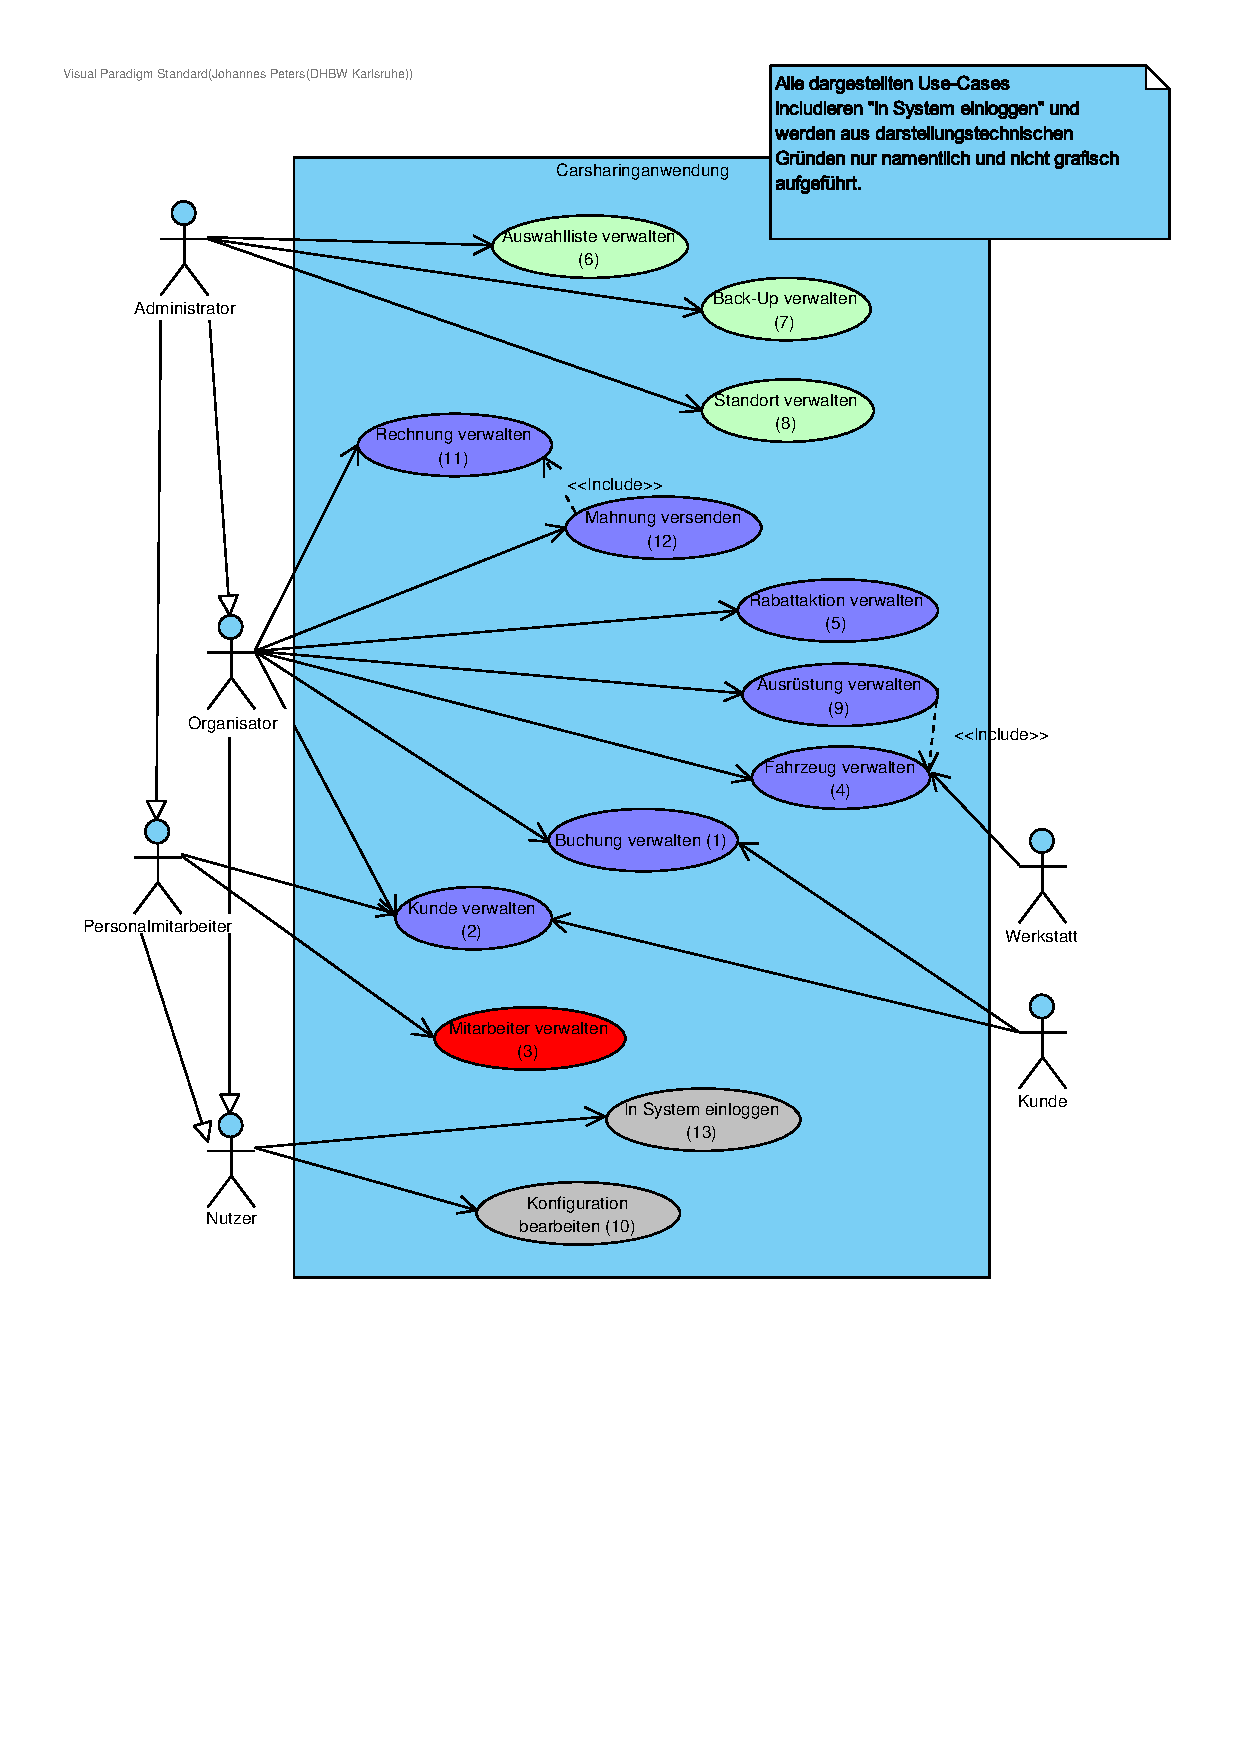
\includegraphics[width=\textwidth, trim = 0cm 8cm 0cm 0cm]{Bilder/Diagramme/Use-Case Diagramm.pdf}
    \caption{Use-Case Diagramm}
    \label{img:use_case_overview}
\end{figure}


\begin{figure}[!ht]
    \centering
    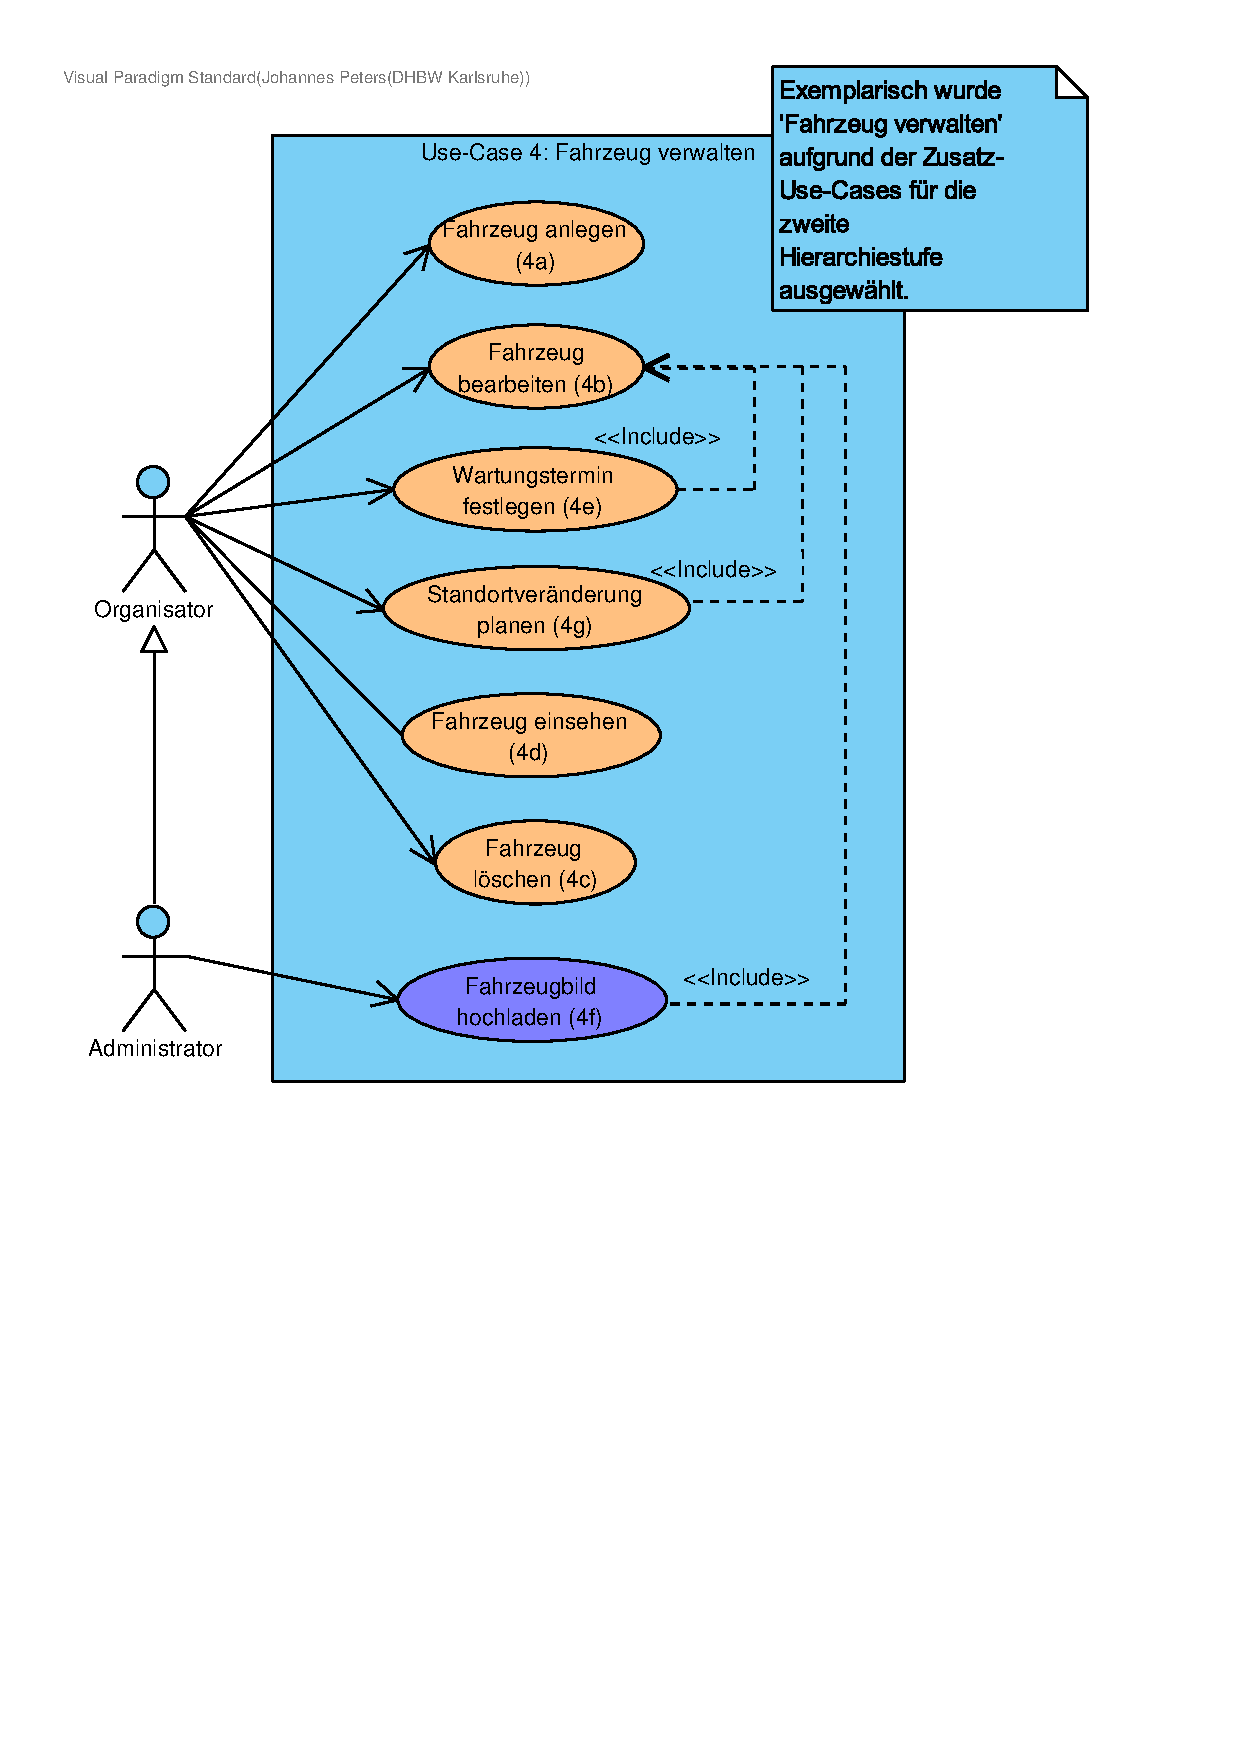
\includegraphics[width=\textwidth, trim = 0cm 11cm 0cm 0cm]{Bilder/Diagramme/Use Case 4_ Fahrzeug verwalten.pdf}
    \caption{Use-Case 4: Fahrzeug verwalten}
    \label{img:use_case_4}
\end{figure}

\chapter{Analyse-Klassen-Diagramm}

In diesem Kapitel wird zuerst auf die Klassen, welche für die Implementierung nötig sind, eingegangen bevor die Abhängigkeiten zwischen diesen Klassen nochmal übersichtlich mittel eines Analyse-Klassen-Diagramms dargestellt werden.

\section{Klassen}
\begin{multicols}{2}
\begin{itemize}
    \item Kunde
    \item Adresse
    \item Vertrag
    \item Mitarbeiter
    \item Rolle
    \item Buchung
    \item Fahrzeug
    \item Fahrzeugklasse
    \item Bild
    \item Reifensatz
    \item Reifen
    \item Kennzeichen
    \item Ausrüstung
    \item Rechnung
    \item Mahnung
    \item Standort
    \item Filiale
    \item Rabattaktion
    \item Backup
    \item Hundetransportbox
\end{itemize}
\end{multicols}

\newpage

\section{Diagramm}

\begin{figure}[!ht]
    \centering
    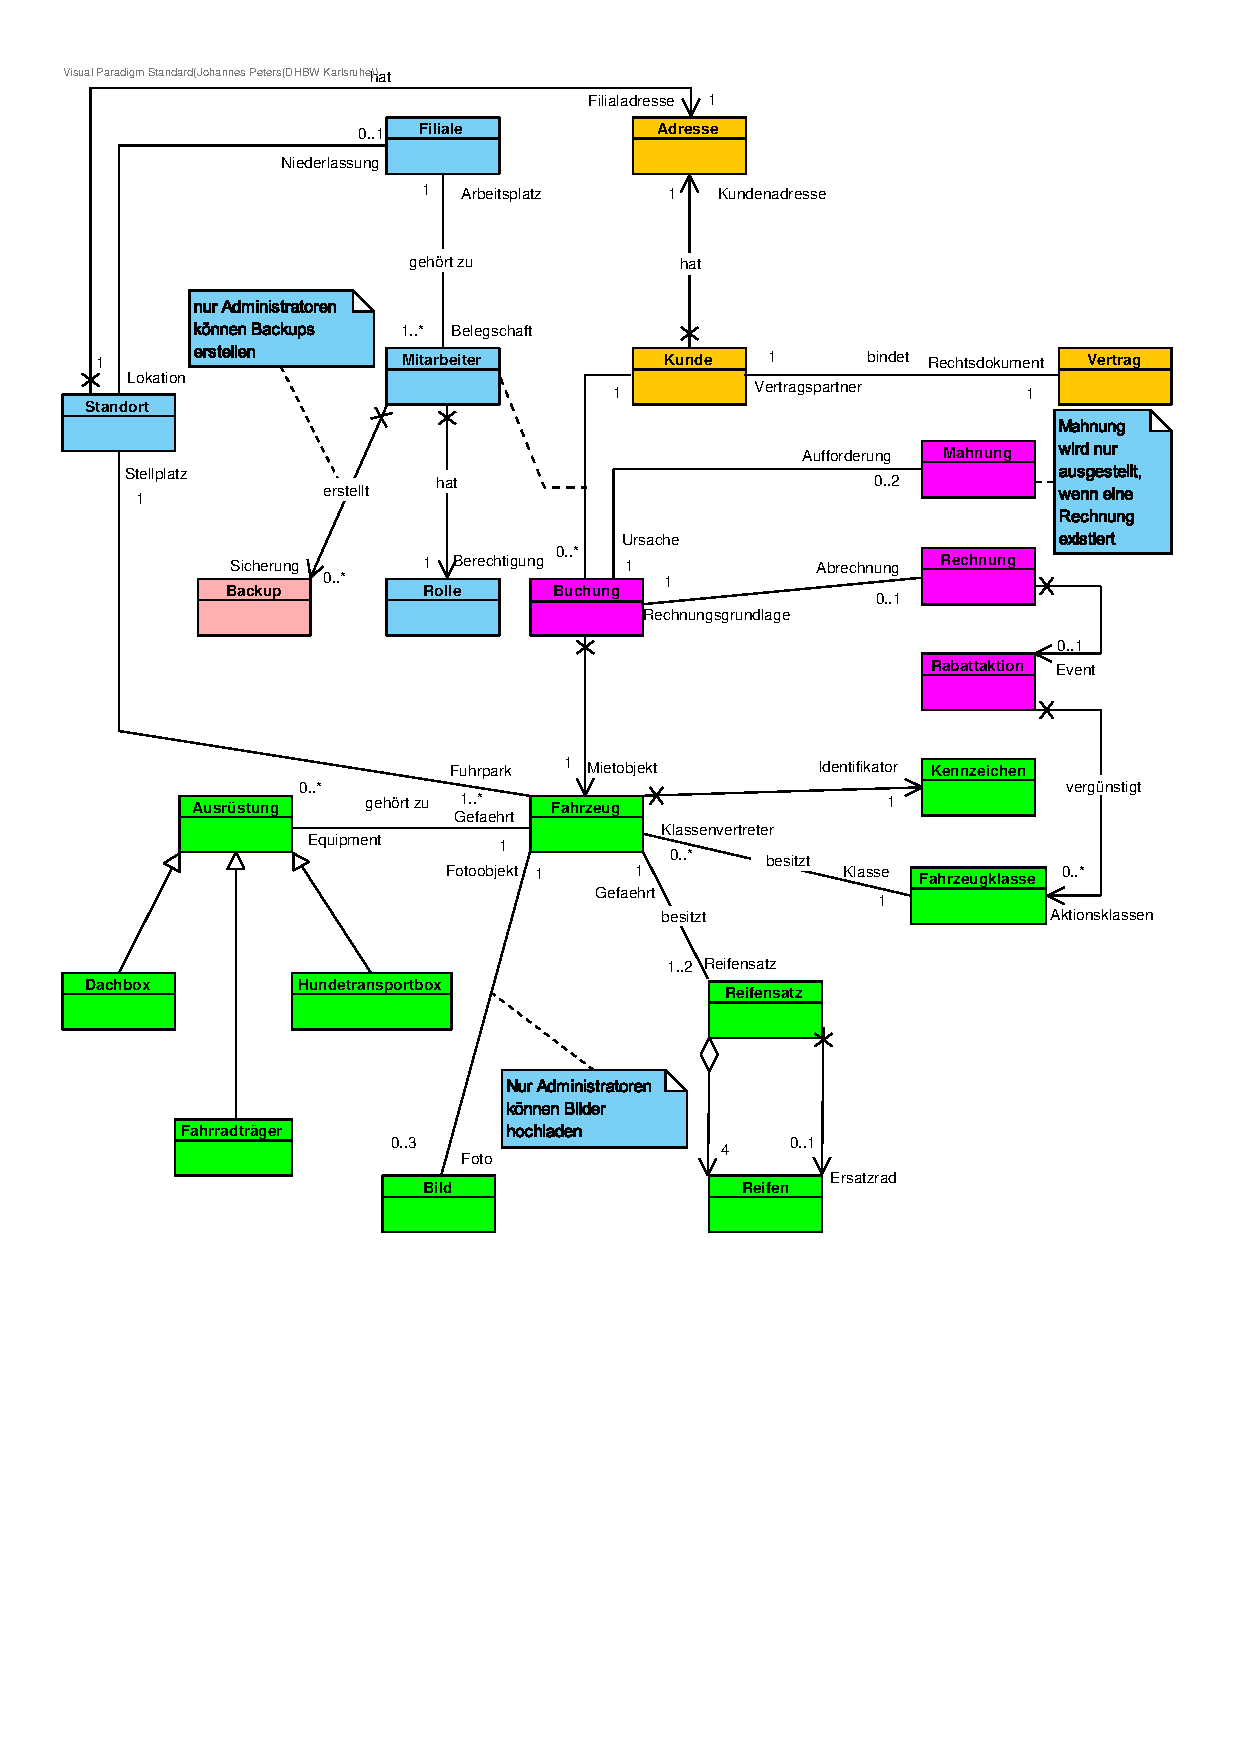
\includegraphics[width=\textwidth, trim = 0cm 9cm 0cm 0cm]{Bilder/Diagramme/Analyseklassendiagramm_v2.pdf}
    \caption{Analyseklassendiagramm}
    \label{img:akd}
\end{figure}

\newpage

\textbf{Kunde}: Sobald sich ein neuer Kunde in einer der Filialen registieren lässt, wird ein neuer Kunde angelegt. Die Kunden-Klasse führt alle nötigen Informationen zur Identifikation und Ausstellung von Rechnungen als Attribute zusammen. Von diesen Informationen sind Finanzdaten ausgenommen, da diese laut Anforderung durch ein anderes System verwaltet werden. Zu den Identifikationsinformationen gehört eine Anschrift, welche durch eine Referenz auf die Adresse-Klasse eingebracht wird. 

Dabei kann jeder Kunde nur eine Adresse haben. Umgekehrt könnte zwar auch die gleiche Adresse auf mehrere Kunden verweisen (z.B. wenn mehrere Kunden im selben Haus wohnen wie es bei einer Familie der Fall sein könnte), doch ist diese Referenz für das Programm unwichtig und somit wird die Assoziation nur unidirektional dargestellt. 

Für eine rechtliche Grundlage muss jeder Kunde einen Vertrag unterzeichnen, der digital eingescannt und abgespeichert werden soll. Die bidirektionale Verbindung weist jedem Kunden genau einen Kundenvertrag zu und natürlich wurde jeder Kundenvertrag von nur einem Kunden unterzeichnet. 

Ein Kunde kann mehrere Buchungen durchführen, die er aber zum aktuellen Projektstand nicht selbst tätigen soll. Der Kunde äußert einen Kundenwunsch an einen Mitarbeiter und der Mitarbeiter legt für den Kunden eine Buchung an, die auf den Kunden verweist. Ein Kunde darf mehrere Buchungen anlegen lassen, aber eine Buchung verweist nur auf einen Kunden. Aus diesem Grund fungiert die Mitarbeiter-Klasse als Koordinator.  

\textbf{Adresse}: Die Adresse wird in Straße, Hausnummer, Wohnungszusatz, Ort und Postleitzahl aufgeteilt. Mit der Adress-Klasse werden die Adressen der Kunden und Filialen dargestellt. Da die Adresse-Klasse jeweils nur als Bestandteil anderer Klassen fungiert sind alle Assoziationen unidirektional auf die Adress-Klasse verweisend. 

\textbf{Vertrag}: Die Vertrags-Klasse bildet die Verträge ab, welche die Kunden bindet. Der Vertrag soll unterschieben eingescannt und als PDF-Datei im System abgelegt werden. Die einzigen zusätzlichen Angaben sind der Pfad und ein Vertragsdatum. Ein extra Dateiname wird nicht abgespeichert, da dieser dem Dateipfad entnommen werden kann.

\textbf{Mitarbeiter}: Die Klasse 'Mitarbeiter' stellt die Mitarbeiter des Unternehmens dar. Die Darstellung eines Mitarbeiters im System dient der Zugriffsbeschränkung der Anwendung mittels Rollen und der Identifikation von im System eingetragene Veränderungen. Jedem Mitarbeiter wird unidirektional eine Rolle zugewiesen. Da die Anwendung nicht auf Basis einer Datenbank arbeitet und auf Abfragen wie die Gruppierung der Mitarbeiter nach vergebenen Rollen irrelevant ist, wurde nur eine unidirektionale und keine bidirektionale Assoziation angenommen.

Jeder Mitarbeiter hat einen festen Arbeitsplatz, welcher durch eine Referennz auf die Klasse 'Filiale' gekennzeichnet ist. Umgekehrt sind in einer Filiale mehrere Mitarbeiter beschäftigt. 

Bereits bei der Klasse 'Kunde' angesprochen fungiert der Mitarbeiter als Koordinator zwischen Kunde und Buchung. 

Weiterhin können Mitarbeiter, unter der Einschränkung, dass der Mitarbeiter die 'Admin'-Rolle hat, Backups erstellen. Der Ausdruck 'können' impliziert, dass nicht jeder Mitarbeiter ein Backup anlegt und dass auch auch der selbe Mitarbeiter mehrere Backups erstellen kann. 

\textbf{Rolle}: Mit den Rollen sollen die Rechte innerhalb der Anwendung verteilt werden können. Dazu stellt die Klasse 'Rolle' neben dem Rollennamen für alle Funktionen der Anwendung jeweils ein Attribut bereit, welches vom Datentyp Boolean ist und angibt, ob ein Nutzer mit dieser Rolle Zugriff auf die entsprechende Funktion bzw. auf eine GUI-Komponente haben soll. Die Klasse 'Rolle' referenziert keine anderen Klassen, sondern wird nur von der Klasse 'Mitarbeiter' referenziert.

\textbf{Buchung}: Die Klasse 'Buchung' stellt einen vereinbarten Termin für die Mietung eines Autos dar. Dazu wird der Mitarbeiter, welcher die Buchung angelegt hat zusammen mit dem Kunden und dem Datum sowie der Uhrzeit des Termins gespeichert. Außerdem steht die Klasse 'Buchung' in Assoziation mit der Fahrzeug-Klasse, um festlegen zu können, welches Fahrzeug gemietet werden soll. Pro Buchung soll ein Kunde nur ein einziges Fahrzeug buchen können.

Da bei einer Buchung eines Fahrzeugs der Preis durch Rabattaktionen beeinflusst werden kann, steht die Buchungs-Klasse in Assoziation mit der Klasse 'Rabattaktion'. Um den Preis zufälligerweise durch mehrere Rabattaktionen nicht mehrfach zu drücken, soll pro Buchung wenn überhaupt nur eine einzige Rabattaktion einbezogen werden.

Nach Abschluss einer Fahrt bzw. nach Ablauf eines Buchungszeitraums wird automatisch eine Rechnung erstellt. Die dadurch entstehende Assoziation zwischen Buchung und Rechnung ist bidirektional. Eine Buchung weist entweder keine Rechnung vor, solange der Termin noch offen ist oder genau eine Rechnung, wenn der Termin abgeschlossen wurde.

Sofern die Rechnung im vorgegebenene Zeitrahmen beglichen wird, ist damit der Buchungsvorgang abgeschlossen, doch sollte eine Zahlung überfällig sein, erzeugt das System auf Basis der Buchung eine oder zwei Mahnungen. Jede Mahnung verweist dabei eindeutig auf die zugehörige Buchung. Eine dritte Mahnung wird nicht ausgestellt, denn anstelle dieser soll das schweizer Bankkonto eingefroren werden und andere rechtliche Schritte werden eingeleitet. 


\textbf{Fahrzeug}: Die Klasse Fahrzeuge ist für das Abbilden der Fahrzeuge zuständig und das Kernobjekt der Anwendung. Jedem Fahrzeug wird genau eine Fahrzeugklasse zugeordnet und in diesem Fall ist die Assoziation bidirektional, da umgekehrt z.B. auch eine Suche nach Fahrzeugen einer bestimmten Fahrzeugklasse möglich sein soll.

Jedes Fahrzeug im Fuhrpark des Unternehmens benötigt eine rechtlich eindeutige Identifikation mittels Nummernschild, weshalb jedes Fahrzeug auf genau ein Kennzeichen verweist. Eine umgekehrte Verknüpfung ist nicht nötig für ein einfaches Buchungssystem. 

Um die Fahrtüchtigkeit der Fahrzeuge zu allen Jahreszeiten gewährleisten zu können, müssen die Fahrzeuge mit den passenden Saisonreifen ausgerüstet sein. Um dies im Überblick zu behalten, verweist ein Fahrzeug auf einen Reifensatz. Jedes Fahrzeug hat einen Sommer- und Winterreifensatz. Um die Zuordnung zu genau dem zugehörigen Fahrzeug sicherzustellen, ist die Verbindung bidirektional. 

Für ein optisch ansprechendes GUI gibt es die Möglichkeit beim Anlegen eines neuen Fahrzeuges auch ein oder mehrere Bilder hochzuladen. Dieses Angebot ist optional und sollte kein Bild hochgeladen werden, dann wird ein 'Placeholder'-Bild eingefügt. Das Hochladen von Bildern ist nach Aufgabenanalyse und -anforderung ebenfalls als eine Administratorfunktion deklariert. Um nicht übermäßig viele Bilder hochzuladen, ist ein Limit auf drei Bilder gesetzt. 

Beim Ausleihen der Fahrzeuge für besondere Anlässe kann es auch sein, dass zusätzliche Ausrüstung erwünscht ist. Die Verbindung zur Ausrüstung ist als bidirektional gewählt, nicht nur vom Fahrzeug aus ersichtlich sein soll welche Ausrüstung vorhanden ist, sondern auch um zu verhindern, dass die selbe Ausrüstung im System ausversehen auf mehreren Fahrzeugen angebracht werden soll. 

Die letzte Assoziation für ein Fahrzeug verweist auf den Standort. Um ein Fahrzeug zu buchen, muss bekannt sein, wo dieses Fahrzeug parkt. Von der andern Seite aus betrachtet gibt es am Standort nur eine gewisse Anzahl an Parkplätzen, sodass bekannt sein muss, welche Fahrzeuge sich zu dem bestimmten Zeitpunkt vor Ort befinden. 

\textbf{Fahrzeugklasse}: Die Fahrzeugklassen sind für das Unterteilen der Fahrzeuge in verschiedene Kategorien zuständig. Diese Kategorien werden mit der Klasse 'Fahrzeugklasse' dargestellt. Eine Kategorie zeichnet sich dabei durch einen Namen, einen Preis und den benötigten Führerschein aus. Solch einer Kategorie sind beliebig viele Fahrzeuge zugeordnet. Dabei ist es denkbar, dass eine Fahrzeugklasse existiert, das Carsharing-Unternehmen aber keinen Klassenvertreter im Fuhrpark besitzt. 

\textbf{Bild}: Die Klasse Bild stellt die Bilder der Fahrzeuge dar. Jedes Bild ist einem Fahrzeug zugeordnet. Als weitere Attribute besitzt diese Klasse den Titel des Bildes sowie den Pfad, an welchem das Bild liegt.

\textbf{Reifensatz}: Ein Reifensatz dient der Unterscheidung zwischen Sommer- und Winterreifen und verweist auf ein bestimmtes, zugehöriges Fahrzeug, sodass jedes Fahrzeug zwei Reifensätze haben sollte. Da es z.B. auch Ganzjahresreifen gibt, kann ein Fahrzeug entweder ein oder zwei Reifensätze vorweisen.  
Jeder Reifensatz besteht aus vier Reifen und potenziell einem weiteren Reifen (Ersatzreifen).

\textbf{Reifen}: Die Klasse Reifen stellt die Reifen der Fahrzeuge dar. Ein Reifen wird hierbei durch den Hersteller, das Modell, den Zeitpunkt der Herstellung, die Profiltiefe, Saison und die Fahrtrichtung beschrieben.

\textbf{Kennzeichen}: Das Kennzeichen dient der Identifikation eines Fahrzeugs. Um das Kennzeichen eines Fahrzeugs in der Anwendung darzustellen wird die Klasse 'Kennzeichen' implementiert, welche die Zulassungsstelle, die Art des Kennzeichens und eine Zeichenkette für das eigentliche Kennzeichen als Attribute enthält.

\textbf{Rechnung}: Eine Rechnung fällt immer nach dem Abschluss einer Fahrt an. Die Klasse 'Rechnung' bildet solch eine Rechnung ab und beinhaltet Methoden um basierend auf der Buchung eine Rechnung in Form eines PDF-Dokuments zu erstellen und an den Kunden per E-Mail zu versenden. Solch eine Rechnung referenziert dabei immer auf die zugrundeliegende Buchung.

\textbf{Mahnung}: Wenn der Kunde die Rechnung nicht im vorgegebenen Zeitraum begleicht, wird eine Mahnung versendet. Die Klasse 'Mahnung' bildet solch eine Mahnung ab und beinhaltet Methoden, um basierend auf der Buchung eine Mahnung zu erstellen und um diese anschließend an den Kunden zu versenden. Ähnlich der Erstellung einer Rechnung wird ein PDF-Dokument erzeugt, welches im Fall einer Mahnung jedoch manuell ausgedruckt und mittels Post versendet wird. Da eine Mahnung stets auf einer Buchung basiert, wird die zugrundeliegende Buchung referenziert.

\textbf{Standort}: Das Unternehmen ist an verschiedensten Standorten tätig. Grundlegend ist ein Standort eine Betriebsfläche des Carsharing-Unternehmens und ist in allen Fällen eine Lokation, an der Fahrzeuge ausgeliehen werden können. Die Anzahl der Fahrzeuge ist hierbei nicht beschränkt.

Damit der Standort für die Kunden erreichbar ist, wird eine Adresse vorausgesetzt, auf die eine Klasseninstanz des Standortes wie auch bei Kunde unidirektional verweist. 

Es ist bei größeren oder wichtigeren Standorten möglich, dass sich dort auch eine Filiale des Unternehmens befindet, an die sich Kunden wenden können. Ein Standort \textbf{kann} eine Filiale referenzieren, doch umgekehrt \textbf{muss} eine Filiale allein wegen der Adressreferenz auf einen Standort verweisen.

Des Weiteren wird der Standort durch eine Beschreibung und einen Namen beschrieben. 

\textbf{Filiale}: Die Klasse 'Filiale' stellt eine Filiale des Unternehmens dar. Dafür wird die Filiale mit dem Standort in Assoziation gesetzt.

In jeder Filiale sind Mitarbeiter des Unternehmens angestellt. Das heißt, dass die Belegschaft einer Filiale mindestens ein Mitarbeiter ist, wobei theoretisch nach oben keine Schranke gesetzt ist. Als wichtige Information hat diese Klasse das Attribut 'Öffnungszeiten'. 

\textbf{Rabattaktion}: Mit der Klasse 'Rabattaktion' werden die Rabattaktionen dargestellt. Dazu besitzt diese Klasse den prozentualen Preisnachlass und den Namen der Rabattaktion als Attribute. 

Es ist möglich, dass z.B. der Rabatt nicht global auf alle Fahrzeuge gewährleistet werden soll, sondern auf einzelen oder mehrere Fahrzeugklassen. Die dabei entstehende Assoziation ist unidirektional, da eine Rabattaktion auf Fahrzeugklassen verweist, doch die Fahrzeugklasse nichts von einer Verbindung zu eine Rabattaktion kennen muss, da der Preisnachlass erst zur Rechnung erstellt wird. 

\textbf{Backup}: Die Klasse Backup ist für die Darstellung der Backups zuständig. Dafür wird zum einen das Datum und die Uhrzeit der Erstellung des Backups und zum anderen der Pfad, unter welchem das Backup abgelegt wurde, als Attribut bereitgestellt. Es gab die Überlegung, ob auch noch der Mitarbeiter verknüpft werden soll, der das Backup anlegt, doch muss diese Aufgabe nicht vom System übernommen werden, da die erstellte Backupdatei im Dateisystem diese Information des Erstellers automatisch speichert. 

\textbf{Ausrüstung}: Die Klasse 'Ausrüstung' umfasst die Ausrüstung eines Fahrzeugs. Dabei handelt es sich nicht um die Ausstattung des Fahrzeugs (Klimaanlage, Panoramaschiebedach, etc.), sondern um Zusätze wie Fahrradträger, Dachbox und Hundetransportbox. Die Klasse 'Ausrüstung' fungiert dabei als Oberklasse der Ausrüstungsgegenstände und besitzt als Attribute die Kompatibilität mit den verschiedenen Fahrzeugen und das Fahrzeug, welches den Gegenstand momentan ausgerüstet hat. Da die Ausrüstung immer einem Fahrzeug zugeordnet ist, wird stets ein Fahrzeug referenziert.

\textbf{Hundetransportbox}: Die Hundetransportbox ist eine der Unterklassen der Ausrüstung, welche die Klasse 'Ausrüstung' um folgende Attribute erweitert: Das Maximalgewicht des Hundes, Höhe, Breite und Länge sowie das Volumen.

\textbf{Fahrradträger}: Ein Fahrradträger ist ebenfalls ein Teil der Ausrüstung und somit eine Unterklasse der Klasse 'Ausrüstung'. Die Klasse Fahrradträger hat zusätzlich Attribute für die Anzahl der Fahrräder, welche mit dem Fahrradträger transportiert werden können, und das maximale Gewicht mit dem der Fahrradträger beladen werden darf.

\textbf{Dachbox}: Die letzte Unterklasse der Ausrüstung ist die Dachbox, welche zusätzlich Attribute für das Volumen und die Größenmaße der Dachbox besitzt.

\chapter{Sequenzdiagramm}

Im Folgenden wird der Vorgang eines vollständigen Buchungsdurchgangs betrachtet, um final mittels Sequenzdiagrammen das Vorgehen visuell darzustellen.

Bei der Erarbeitung wird aufgrund des Umfangs ein Teil der Detailtiefe entfernt. Die exakte Kommunikation mit der Datenbasis (in Realität mit einer Datenbank und im Projekt mit den CSV-Dateien) wird nicht betrachtet. Bei der Interaktion mit der Anwendung wird die Unterteilung in verschiedene GUIs unter dem Begriff 'Benutzeroberfläche' zusammengefasst. Es wird ebenfalls davon ausgegangen, dass für den Sequenzablauf benötigte Datensätze wie Fahrzeuge, Standorte, Kunden und Mitarbeiter bereits vorhanden sind und nicht erst angelegt werden müssen. Davon auszugehen, dass mit einer vollständig leeren Datenbasis begonnen wird ist für die Abbildung des Buchungsablaufs nicht zielführend. Aus diesem Grund wird angenommen, dass ausschließlich die Datenbasis der Buchungen, Rechnungen und Mahnungen leer ist. Weiterhin wird in den Sequenzdiagrammen auf die Verwendung von Funktionen verzichtet und Vorgänge werden umschrieben oder umgangssprachlich aufgeführt.

\section{Aktionsbetrachtung: Buchung eines Fahrzeugs}

Eine Buchung soll angelegt werden. Abgesehen vom eigentlichen Buchungsdurchgangs soll auch die Abrechnung des Buchungstermins einbezogen werden. Ausgehend davon lassen sich mehrere Teil-Abläufe identifizieren: Buchung eines Fahrzeugs, Stornierung einer Buchung, Antreten des gebuchten Termins, Beendigung der Fahrt mit Erstellung einer Rechnung und notfalls Mahnungen. Die Buchung und die Stornierung lassen sich zusammenfassen, gleiches gilt für die Beendigung und die Rechnungsausstellung. Da die Buchung über die Desktopanwendung ausschließlich in der Filiale stattfinden kann, ist ein Akteur der Organisator, der zweite Aktuer ist der Kunde.


Der gesamte Buchungsvorgang beginnt damit, dass ein Kunde die Filiale betritt und einen Termin buchen möchte. Sobald der Kunde einen Terminwunsch und die damit verbundenen Bedinungen (Fahrzeug, Zeitraum, Standort) formuliert, kann der Organisator diese Daten in die Benutzeroberfläche eingeben und die Eingabe validieren lassen. Das System meldet anschließend zurück, ob die Eingabekombination buchbar ist oder nicht.


Die Stornierung eines gebuchten Termins ist bis zu 10 Stunden vor Antritt möglich. Um einen Termin stornieren zu können, muss der Kunde telefonisch oder in Person die Stornierung beim Organisator anfragen. Dieser filtert nach dem Kunden und wählt die betroffene Buchung aus. Sobald die richtige Buchung gefunden wurde, kann sie gelöscht werden.


Beim Terminantritt muss der Kunde seine Kundekarte dem Kartenlesegerät präsentieren, welches zum gebuchten Fahrzeug gehört. Der darin enthaltene Mini-Controller vergleicht die in der Karte enthaltenen Kundendaten mit den Daten in der Datenbasis. Sofern für den Kunden eine Buchung hinterlegt ist, bei der das Fahrzeug und die Zeit übereinstimmen, wird das Fahrzeug vom Controller entsperrt.


Nach der finalen Abgabe überprüft der Controller den Kilometerstand und verriegelt anschließend das Fahrzeug. Serverseitig wird nun der neue Kilometerstand mit dem alten Stand verglichen und daraus wird die gefahrene Kilometeranzahl berechnet. Auf Basis der Buchung (enthält gebuchtes Fahrzeug, welches wieder auf die Preiskalssen verweist) und den Kilometern wird ein Rechnungsobjekt erstellt. Letztendlich erhält der Kunde per E-Mail einen visuellen Export des Rechnungsobjekts.


Der Kunde hat nun standardmäßig 30 Tage Zeit, um die Rechnung zu zahlen. Sollte die Frist versäumt werden, wird die erste Mahnung erstellt und dem Kunden zugesandt. Nach 45 Tagen erfolgt die zweite Mahnung. Sollte nach zwei Monaten die Rechnung immer noch ausstehend sein, wird das betroffene Kundenkonto gesperrt und rechtliche Schritte werden eingeleitet.

\newpage

\section{Pseudo-Code}

\lstinputlisting[style=Pseudocode, caption={Szenario Event anlegen}]{Quellcode/Pseudocode.txt}

\section{Diagramme}

\subsection{Buchung anlegen}


Das Anlegen einer Buchung wird in Abbildung \ref{img:buchung01} auf Seite \pageref{img:buchung01} dargestellt. Die Sequenz beginnt damit, dass der Kunde einen Terminwunsch gegenüber einem Mitarbeiter äußert. Der Organisator öffnet daraufhin das Formular für das Anlegen einer Buchung und teilt dem Kunden mit, dass die Buchung nun entgegengenommen werden kann.

Für die eigentliche Buchung nennt der Kunde dem Organisator zuerst den Zeitraum, den Standort und das Fahrzeug. Der Organisator trägt diese Daten in das Formular ein und klickt anschließend auf 'Buchung überprüfen'. Daraufhin lädt die Anwendung die Fahrzeug-, Standort- sowie Buchungsdaten und gleicht diese mit der Eingabe des Organisators ab. Falls es eine Kollision mit einer anderen Buchung gibt, wird die Buchung abgebrochen. In diesem Fall nennt der Kunde andere Buchungsdaten, bis es keine Kollision mehr gibt. Sollte es keine Kollision geben, wird die Buchung in der Datenbasis hinterlegt und das System bestätigt die Buchung. Daraufhin teilt der Organisator dem Kunden mit, dass die Buchung erfolgreich war.

Optional kann der Kunde die Buchung nun stornieren. Dazu muss der Kunde gegenüber dem Organisator den Wunsch äußern, die Buchung zu stornieren. Der Organisator erfagt daraufhin den Namen des Kunden und gibt diesen in der entsprechenden Suchleiste ein. Die Anwendung lädt daraufhin die Kundendaten aus der Datenbasis und zeigt sie dem Organisator an. Im Anschluss erfagt der Organisator, welche Buchung der Kunde gern stornieren möchte. Nachdem der Kunde die Buchung spezifiziert hat, wählt der Organisator die entsprechende Buchung aus. Daraufhin lädt die Anwendung die Buchungsdaten für die spezifizierte Buchung aus der Datenbasis und zeigt diese Daten an. Der Organisator klickt anschließend auf 'Buchung stornieren', wodurch die Buchung aus der Datenbasis gelöscht wird. Der Organisator erhält darufhin eine Bestätigung für das Löschen der Buchung und teilt dem Kunden mit, dass die Buchung erfolgreich storniert wurde. 

\newpage

\begin{figure}[!ht]
    \centering
    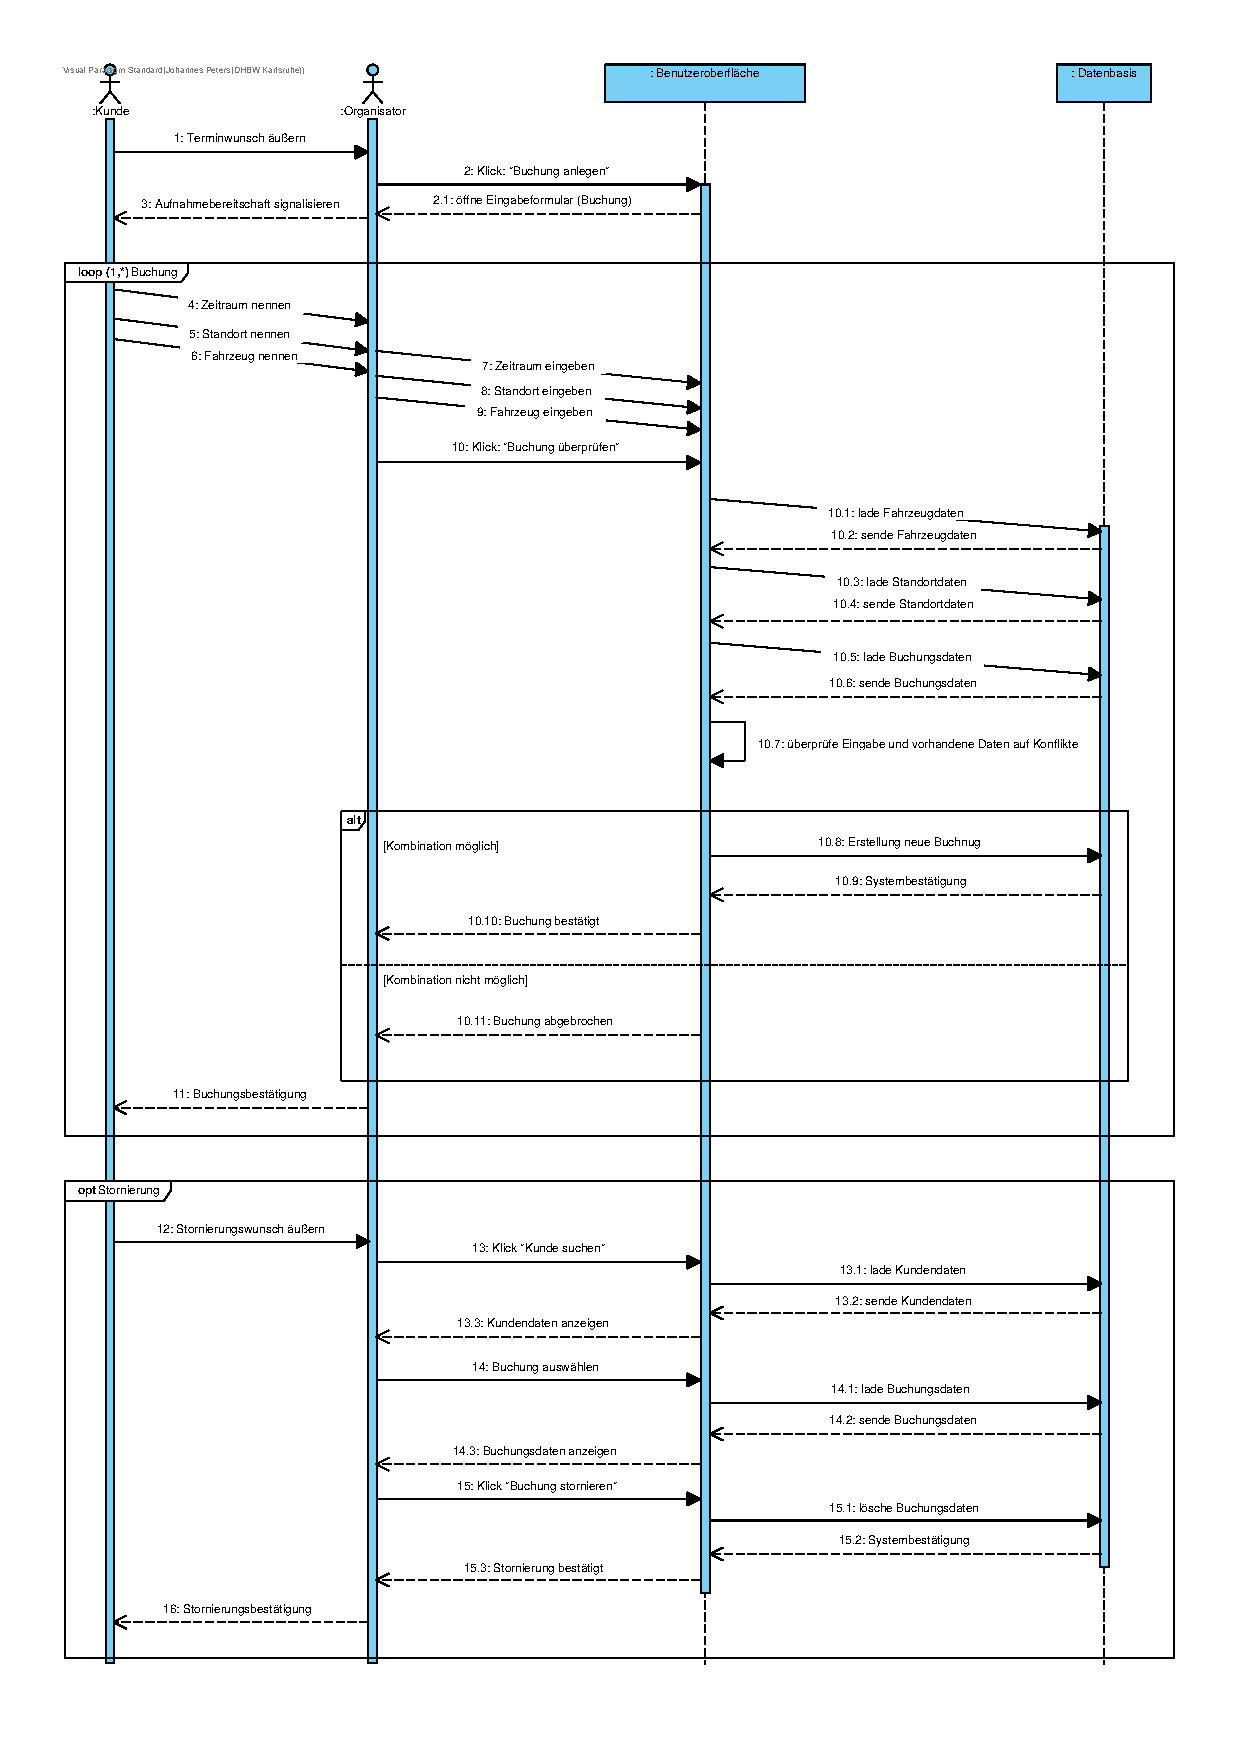
\includegraphics[width=\textwidth, height=\textheight-4cm]{Bilder/Diagramme/SD_Buchungsvorgang_01.pdf}
    \caption{Buchung eines Termins}
    \label{img:buchung01}
\end{figure}


\clearpage

\subsection{Fahrt antreten}

Das Antreten einer Fahrt wird in Abbildung \ref{img:buchung02} auf Seite \pageref{img:buchung02} dargestellt. Hierbei lässt der Kunde zuerst seine Kundenkarte vom Lesegerät einscannen, welches die Kundendaten ausliest und im Anschluss die Buchungsdaten aus der Datenbasis lädt. Nachdem die Buchungsdaten geladen wurden wird zunächst der Standort überprüft, bevor die Kundendaten mit den Buchungsdaten abgeglichen werden. Bei einer übereinstimmung wird zuerst der Kilometerstand für die Abrechnung gespeichert und danach wird das Fahrzeug entriegelt. Nun kann der Kunde seine Fahrt beginnen. 


\begin{figure}[!ht]
    \centering
    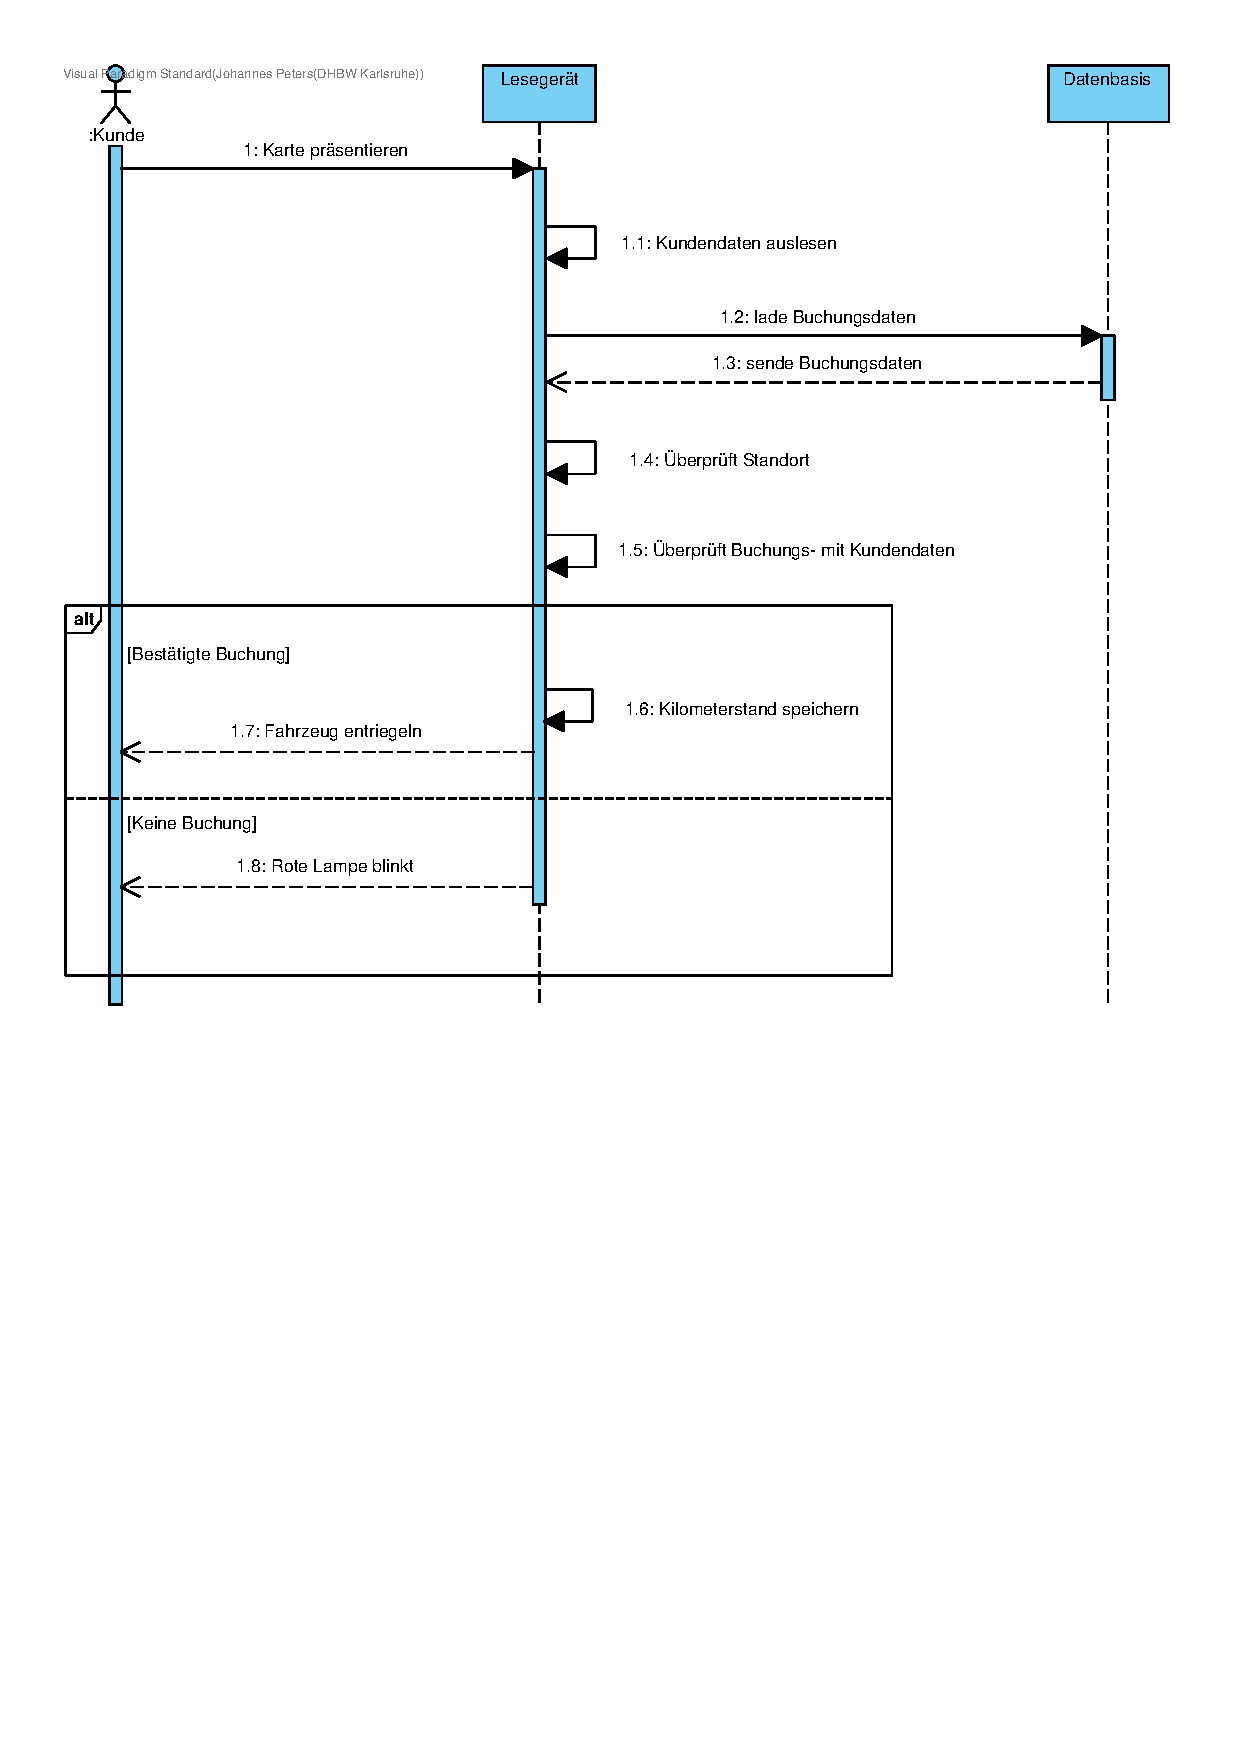
\includegraphics[width=\textwidth, trim = 0cm 13cm 0cm 0cm]{Bilder/Diagramme/SD_Buchungsvorgang_02.pdf}
    \caption{Antritt eines gebuchten Termins}
    \label{img:buchung02}
\end{figure}

\newpage

\subsection{Fahrt beenden}

Das Beenden einer Fahrt wird in Abbildung \ref{img:buchung03} auf Seite \pageref{img:buchung03} dargestellt. Sobald der Kunde das Fahrzeug abstellt wird der Kilometerstand vom Lesegerät abgefragt und das Fahrzeug wird verriegelt. Während der Kunde auf seine Rechnung wartet wird der neue Kilometerstand an den Server gesendet, welcher nach Abfrage des alten Kilometerstands und den Buchungsdaten die gefahrenen Kilometer berechnet. Basierend auf den Buchungsdaten und den gefahrenen Kilometern wird eine Rechnung erstellt, welche vom Server per Mail an den Kunden geschickt wird.


\begin{figure}[!ht]
    \centering
    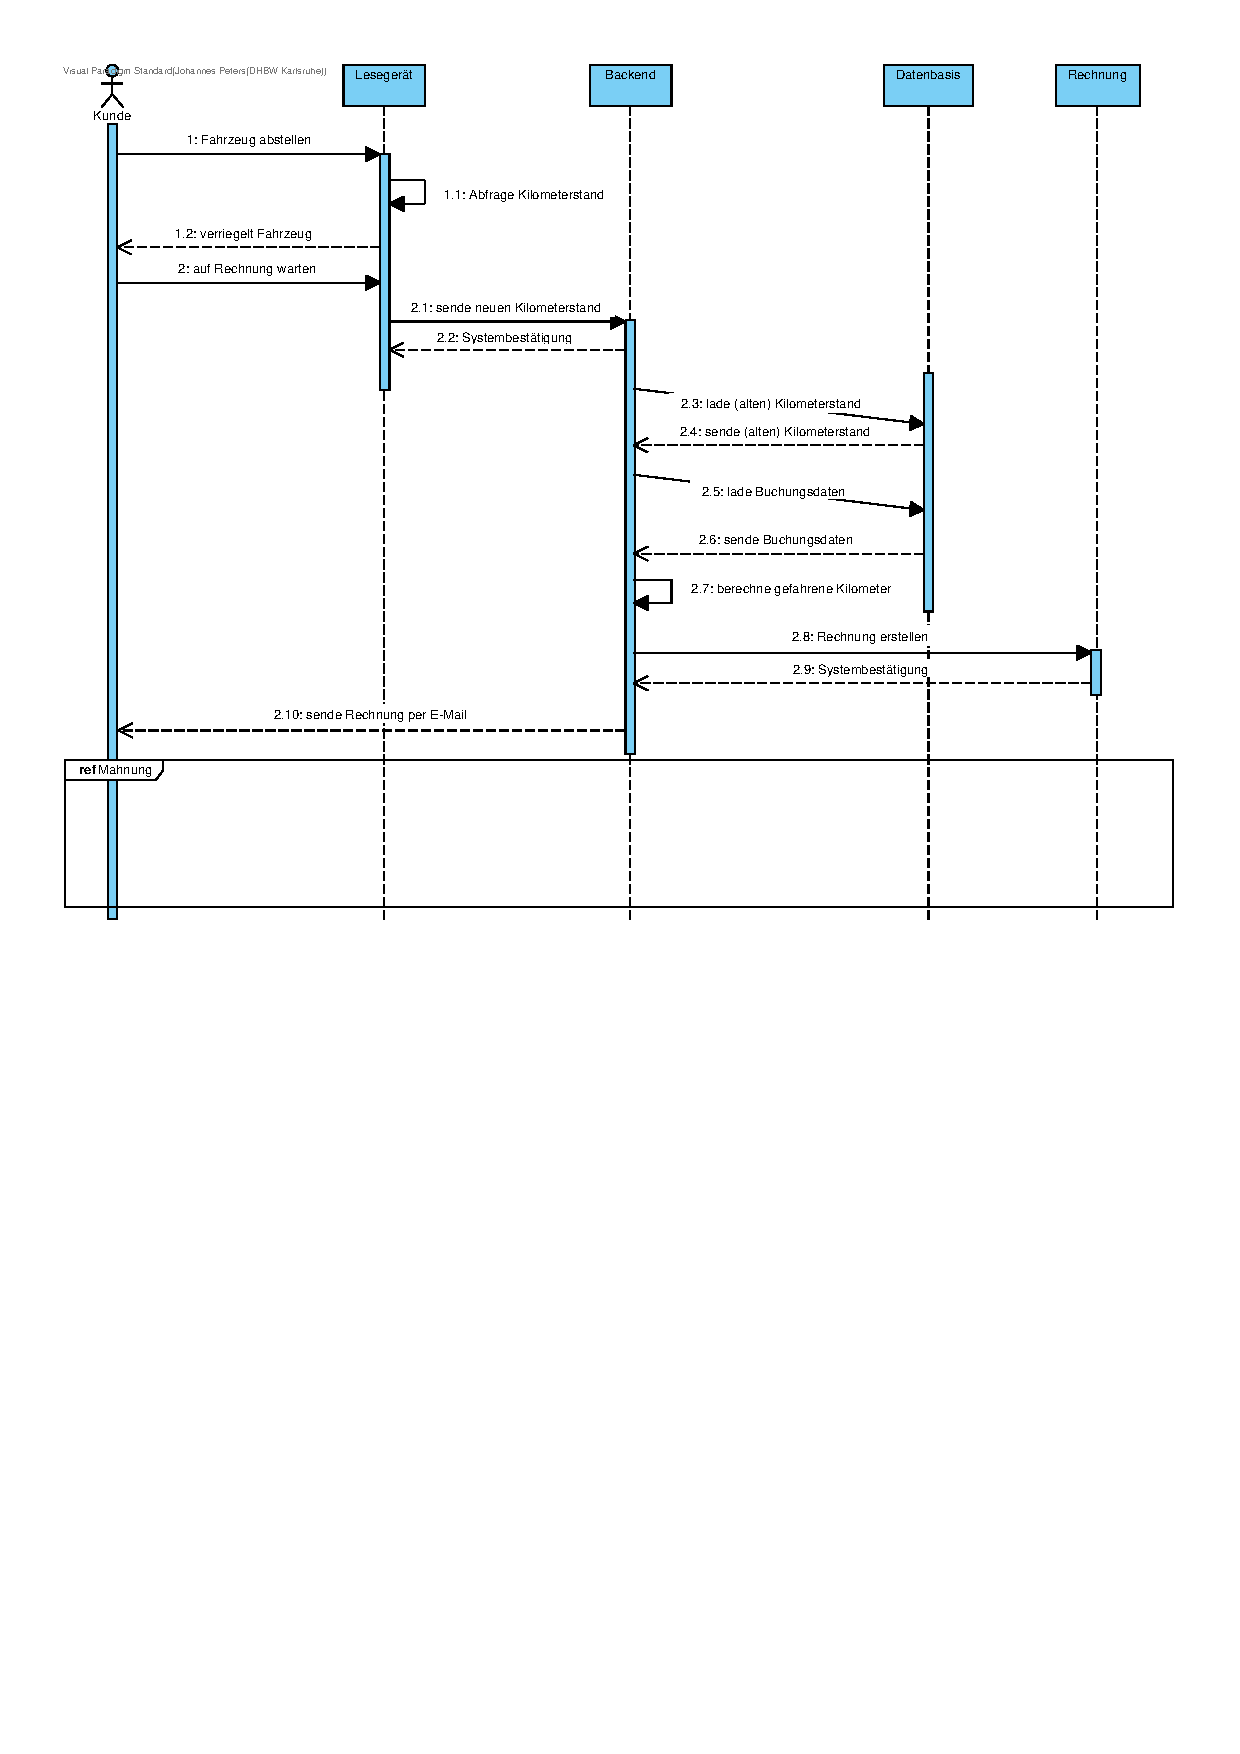
\includegraphics[width=\textwidth, trim = 0cm 14cm 0cm 0cm]{Bilder/Diagramme/SD_Buchungsvorgang_03.pdf}
    \caption{Abschluss eines gebuchten Termins}
    \label{img:buchung03}
\end{figure}

Falls die Rechnung vom Kunden ignoriert wird, erhält der Kunde nach 30 und nach 45 Tagen eine Mahnung. Dies wird in Abbildung \ref{img:buchung03} auf Seite \pageref{img:buchung03} dargestellt. Um eine Mahnung zu versenden lädt der Server zuerst die Rechnungsdaten der überfälligen Rechnung von der Datenbasis.
Im Anschluss erstellt der Server basierend auf der Rechnung eine Mahnung und sendet diese per Mail an den Kunden. Sollte der Kunde nach 60 Tagen nicht gezahlt haben, so wird er für vom Carsharing-Angebot ausgeschlossen. Dazu lädt der Server zuerst die Mahnungsdaten aus der Datenbasis, um den Status der Mahnung zu überprüfen. Wenn die Rechnung zu diesem Zeitpunkt nicht beglichen wurde, werden die Kundendaten aus der Datenbasis geladen und aktualisiert, sodass der Kunde für zukünftige Buchungen gesperrt ist. Sobald der Kunde blockiert ist sendet der Server eine Mail an den Kunden mit der Information, dass der Kunde in Zukunft vom Carsharing-Angebot ausgeschlossen ist und sein Schweizer Bankkonto eingefroren wurde.

\begin{figure}[!ht]
    \centering
    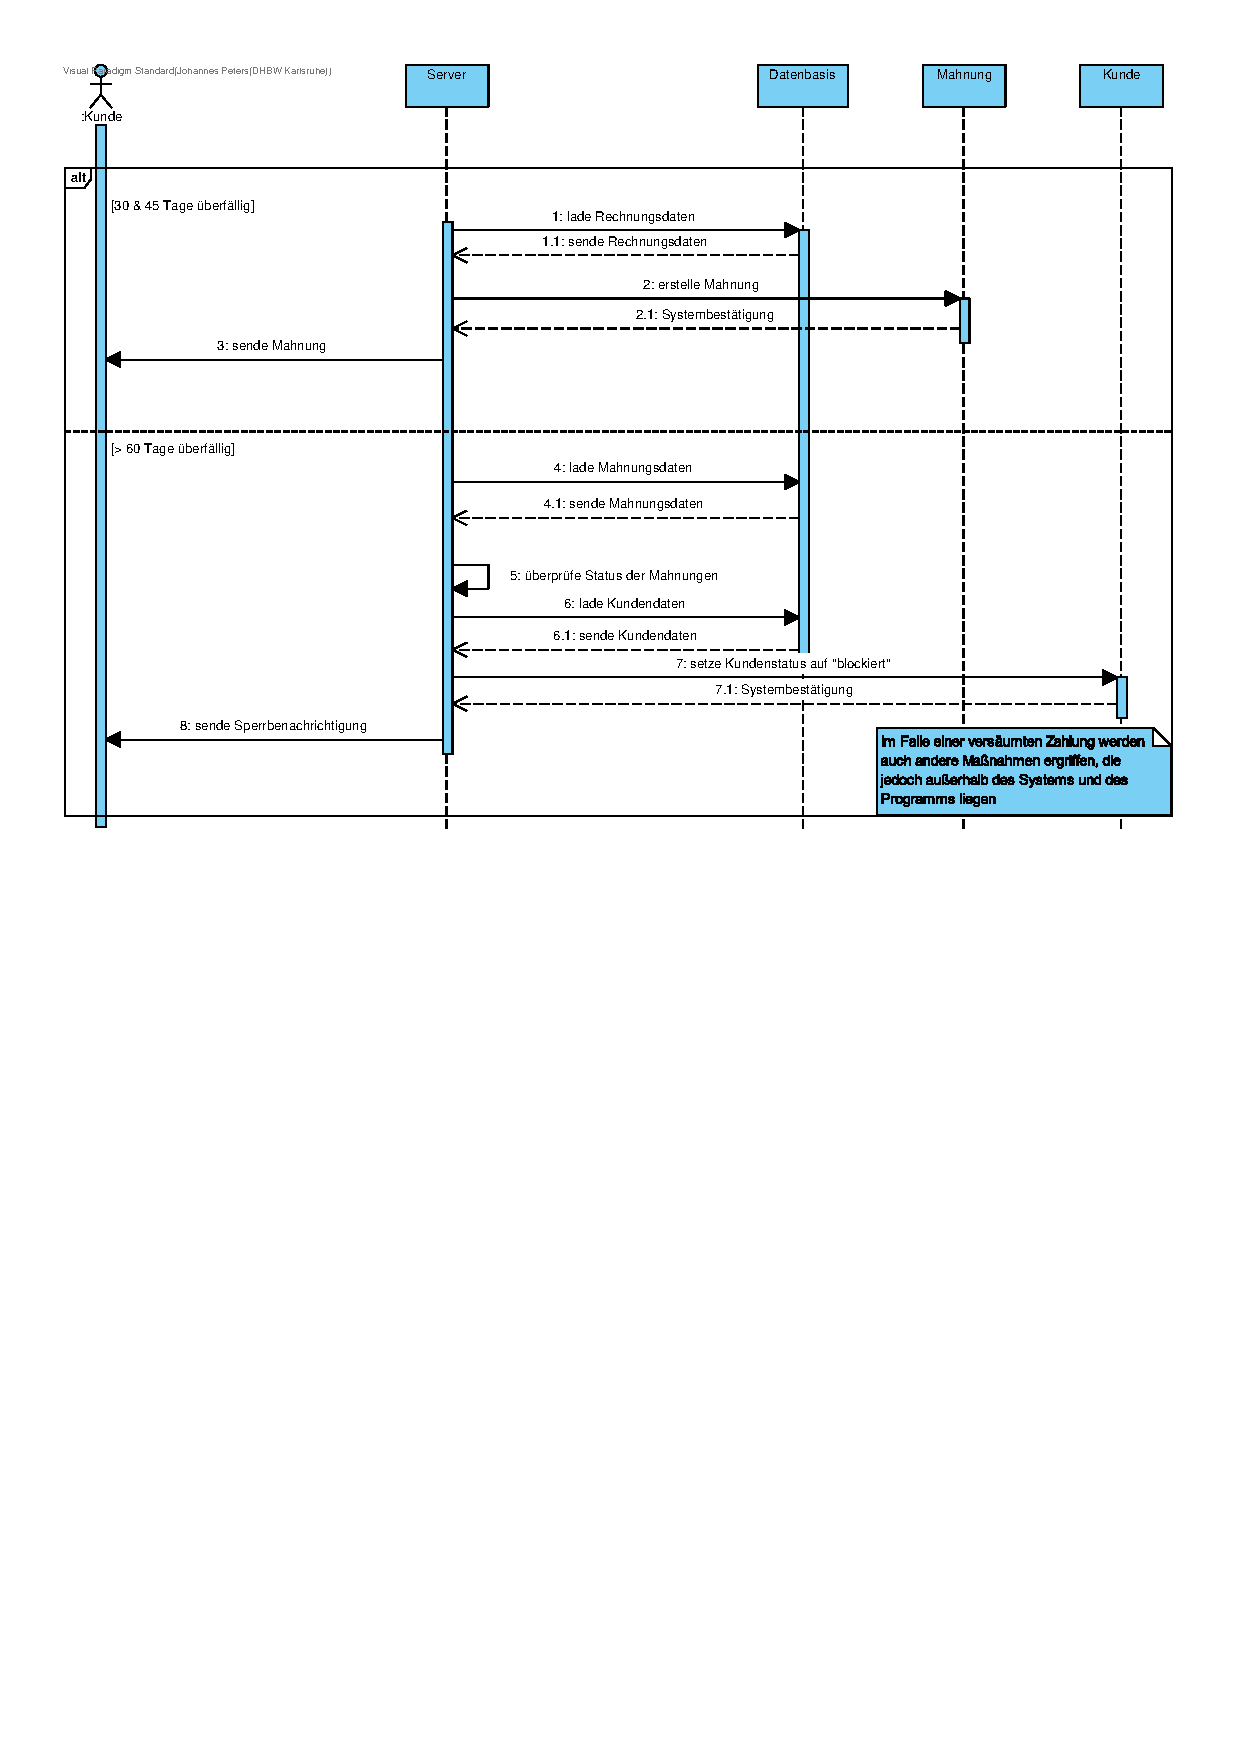
\includegraphics[width=\textwidth, trim = 0cm 16cm 0cm 0cm]{Bilder/Diagramme/SD_Buchungsvorgang_04.pdf}
    \caption{Erstellung der Mahnungen}
    \label{img:buchung04}
\end{figure}

\chapter{Aktivitätsdiagramm}

In diesem Kapitel erfolgt die Erarbeitung der Aktion 'Standort mit neuen Fahrzeugen anlegen' in Form von Aktivitätsdiagrammen. Da hierbei von einer vollständig leeren Datenbasis ausgegangen werden soll, muss jedoch die Aktion aufgegliedert werden. Die Unteraktionen 'Standort anlegen', 'Fahrzeug anlegen' und letztendlich 'Fahrzteug einem Standort zuordnen' müssen somit voneinander getrennt betrachtet werden. 

\section{Pseudo-Code}

\lstinputlisting[style=Pseudocode, caption={Szenario Standort mit Fahrzeugen anlegen}]{Quellcode/AktivitaetsDiagrammPseudo.txt}

\section{Diagramme}

\newpage

\subsection{Standort anlegen}

\begin{figure}[!ht]
    \centering
    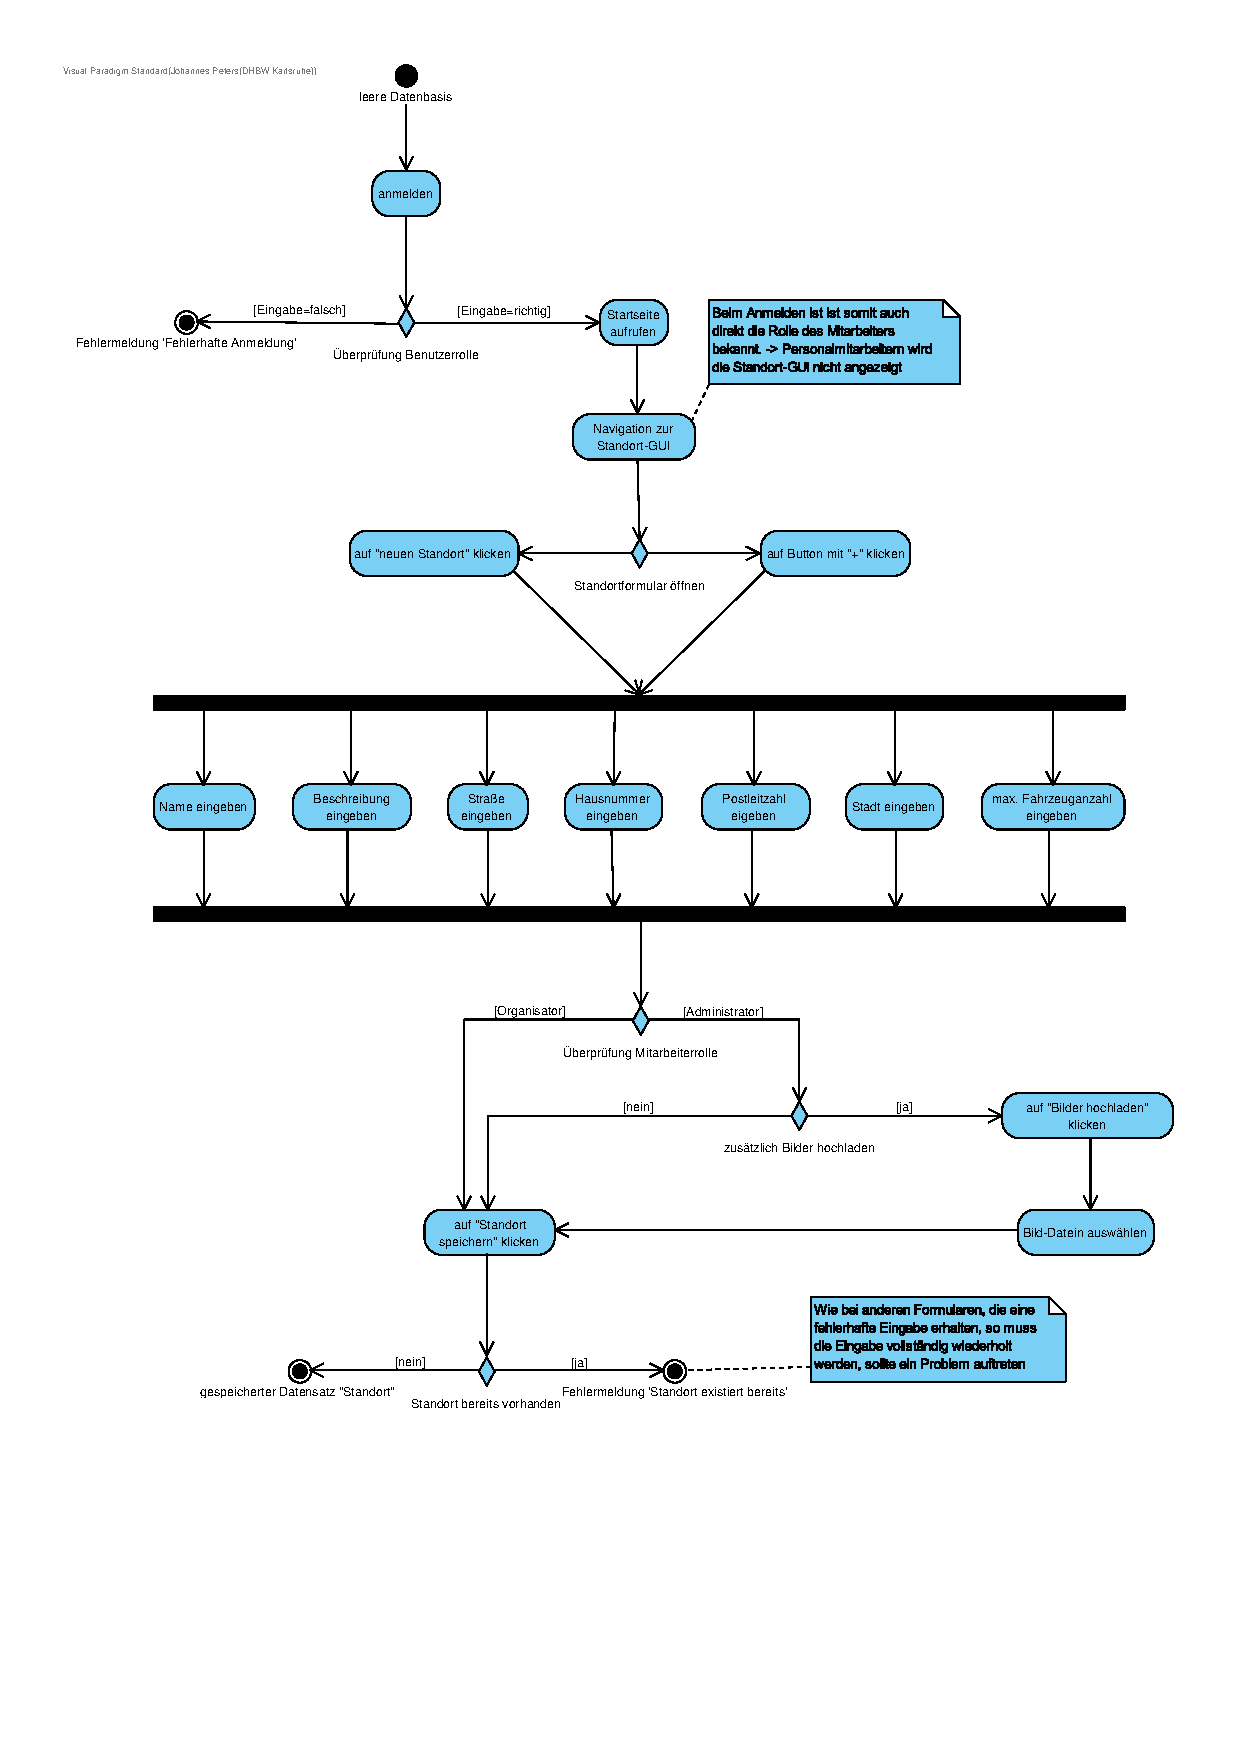
\includegraphics[width=\textwidth, height=\textheight-3cm, trim = 0cm 3cm 0cm 0cm]{Bilder/Diagramme/AD_Standort_anlegen.pdf}
    \caption{Aktivitätsdiagramm: Standort anlegen}
    \label{img:ad_standort}
\end{figure}

Wie bei jeder anderen auf dem System ausgeführten Aktion muss auch beim Anlegen eines neuen Standorts zuerst eine Anmeldung vollzogen werden. Sobald ein Mitarbeiter im System angemeldet ist stehen mittels seines Benutzerprofils auch die Rechte des Nutzers griffbereit. Personalmitarbeiter soll es nicht möglich sein, Standorte anzulegen oder andere Aktionen mit solchen Datensätzen auszuführen, sodass diesen Mitarbeitern eine andere Benutzeroberfläche gezeigt wird wie den Organisatoren und Administratoren. 


Nachdem zu der entsprechenden GUI navigiert wurde und der Mitarbeiter einen neuen Standort anlegen möchte, gibt es zwei Möglichkeiten zum entsprechenden Eingabeformular zu gelangen. Um für die Mitarbeiter, deren IT-Kenntnisse teils mangelhaft sind, mehrere Vorschläge darzustellen gibt es einmal den offensichtlichen Text-Button mit 'neuen Standort anlegen', für die etwas bewanderten Mitarbeiter, zusätzlich einen '+'-Button. Sobald sich das Eingabeformular geöffnet hat, müssen die Felder ausgefüllt werden. 


In welcher Reihenfolge dies ausgeführt wird, ist irrelevant, weshalb im Diagramm diese Aktionen auf parallel dargestellt werden. Sobald alle Texteingaben abgeschlossen wurden, besteht noch die Option Bilder vom Standort hochzuladen, sozusagen ein Titelbild für den Detaileintrag des Standorts. Das Hochladen von Bildern dürfen nur die Administratoren ausführen, sodass zuerst eine Rollenabfrage stattfindet. Sollte ein Administrator diesen Standort anlegen, so wird ihm die Möglichkeit angezeigt und sollte er Bilder hinzufügen möchten, kann er über einen 'Standard-File-Choose-Dialog' Bilder von seinem Computer auswählen und in das Programm laden. Sofern dies erledigt wurde, oder auch nicht, ist es möglich den neuen Standorteintrag zu speichern. 


Bevor der Standort gespeichert wird, erfolgt die Überprüfung, ob dieser Standort bereits vorhanden ist. Sollte das Ergebnis negativ sein, wird der Standort gespeichert. Ist jedoch in der Planung oder Organisation ein Fehler aufgetreten und der Standort exisitiert bereits, erscheint eine Fehlermeldung und die Aktion wird abgebrochen. An sich hätte man im Diagramm anstelle des Endzustandes 'Fehlermeldung' auch eine Schleife einbauen können, die solange läuft wie die Eingabe inkorrekt ist oder bis die Aktion händisch abgebrochen wird. In diesem Fall wird jedoch davon ausgegangen, dass allein auf Basis der Funktionsart eines Eingabeformulars die Eigabefelder geleert werden und die Eingabe wiederholt werden muss. Außer der Abfrage, ob der Standort bereits existiert, findet keine andere logische Überprüfung statt. Sofern sich die Adresse nicht doppelt wird der Datensatz gespeichert. Sollte die Fehlermeldung erscheinen, ist es auch sehr unwahrscheinlich, dass der Mitarbeiter ein zweites Mal die Erstellung des Standortes versucht. 
\newpage

\subsection{Fahrzeug anlegen}

\begin{figure}[!ht]
    \centering
    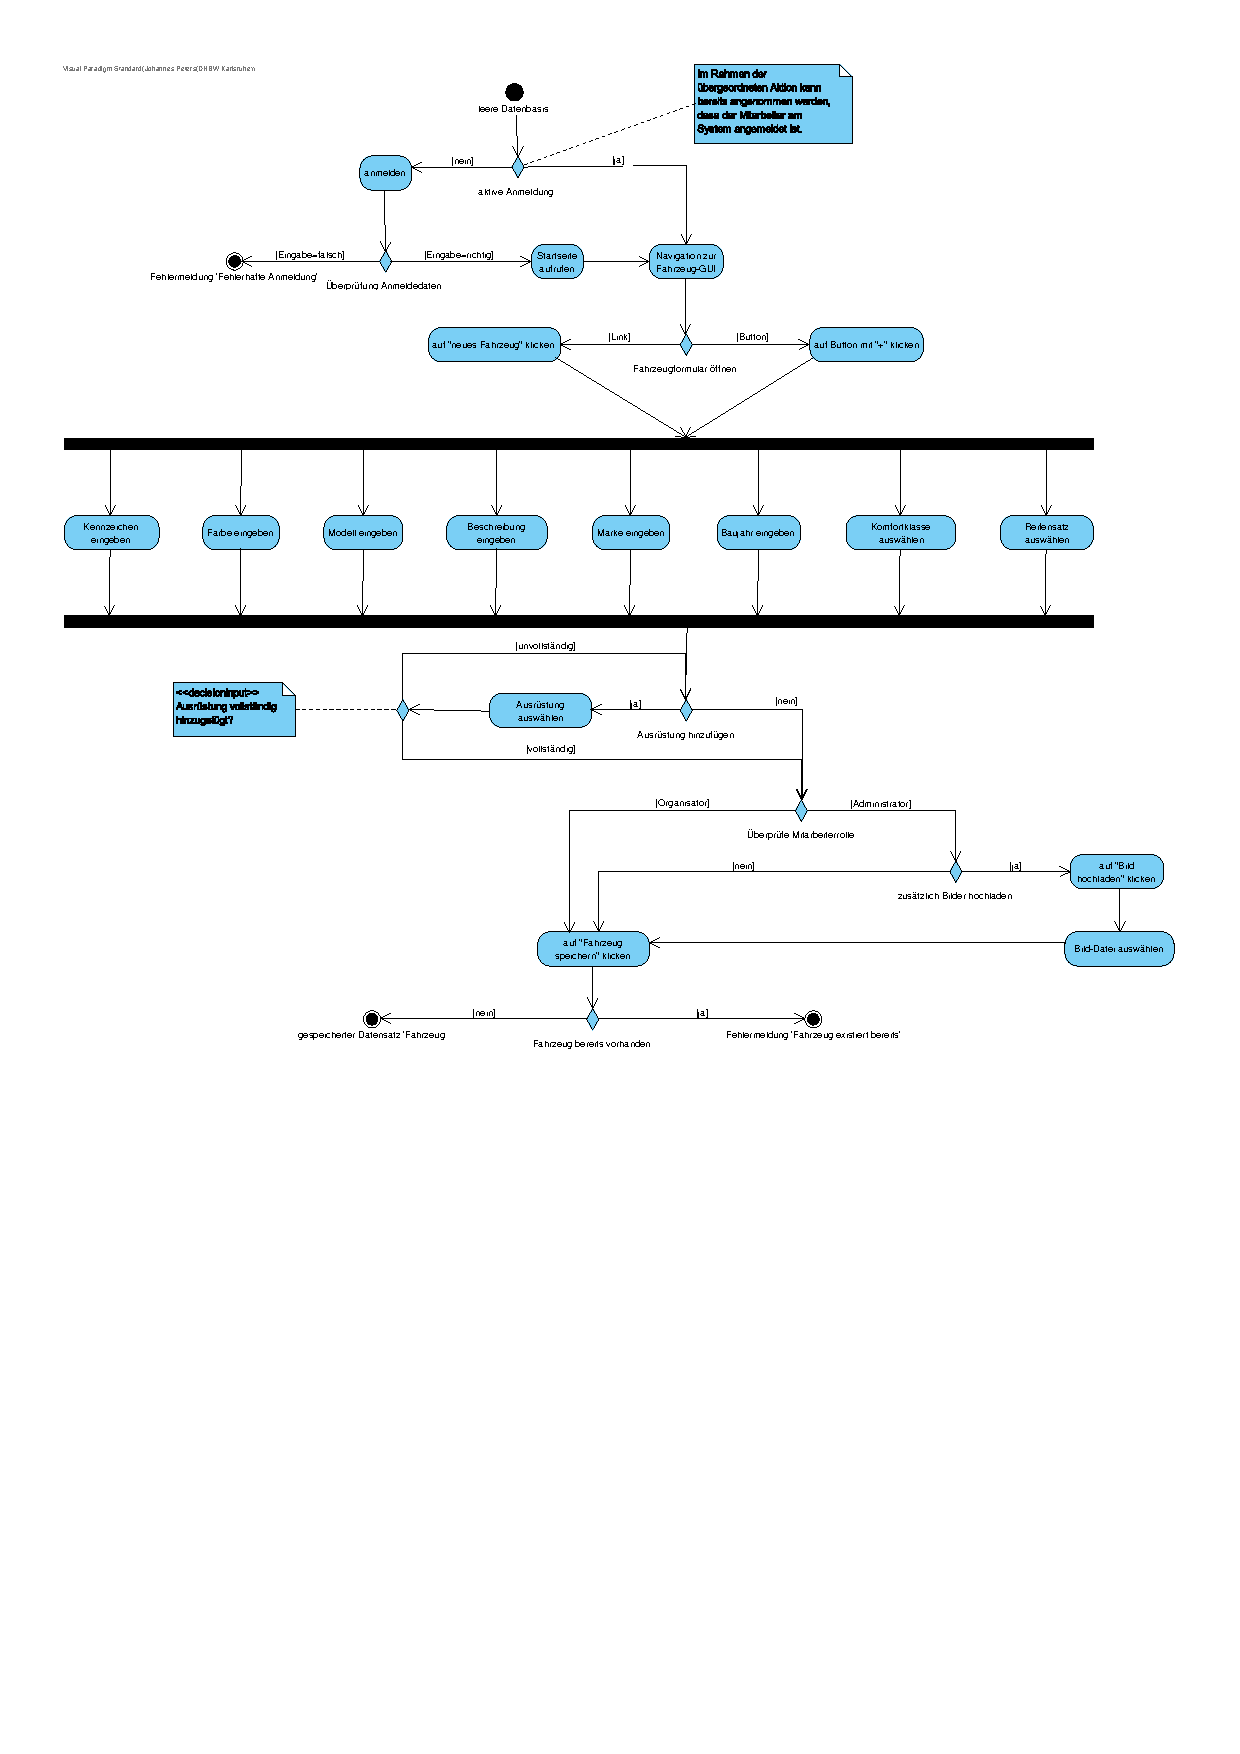
\includegraphics[width=\textwidth, trim = 0cm 11cm 0cm 0cm]{Bilder/Diagramme/AD_Fahrzeug_anlegen.pdf}
    \caption{Aktivitätsdiagramm: Fahrzeug anlegen}
    \label{img:fahrzeug}
\end{figure}

Die eingentliche Aktion, die mit den Aktivitätsdiagrammen analysiert werden soll, ist das Anlegen eines Standortes mit Fahrzeugen. Nur zum besseren Verständnis wurde diese Aktion aufgeteilt, d. h., dass der gesamte Vorgang eigentlich flüssig hintereinander abläuft und der Mitarbeiter, der sich bereits für das Anlegen eines Standortes angemeldet hat, immer noch im System eingeloggt befindet. Theoretisch könnte eine Unterbrechung möglich sein und wurde daher exemplarisch in dieses Diagramm eingebaut. 


Viele Bestandteile des Diagramms sind dem Standort-Diagramm sehr ähnlich, da dass Erstellen und Eingeben von Datensätzen in allen Anwendungsfällen ähnlich ist.


Sollte der Mitarbeiter noch im System tätig sein, so wird er sich bereits irgendwo auf den Benutzeroberflächen befinden und muss sich im Verwaltungsbereich der Anwendung zur Fahrzeug-GUI navigieren. Sollte der Mitarbeiter, aus welchen Gründen auch immer, nicht mehr im System angemeldet sein, so muss dieser sich zuerst wieder anmelden. 


Die Formularbearbeitung ist identisch zum Aufbau bei den Standorten. Da es auch hier irrelevant ist in welcher Reihenfolge die Daten eingegeben werden, wird Parallelisierung verwendet, um dies darzustellen. Die meisten Eingabeaktionen enthalten "eingeben", doch gibt es einige Aktionen, die "auswählen" lauten und somit eine Auswahlmöglichkeit in Form von Drop-Down-Listen implizieren.


Einem Fahrzeug kann Ausrüstung hinzugefügt werden, was durch eine Decision-Node dargestellt wird. Da die Ausrüstung von Fahrzeugen aus Objekten wie Fahrradträger, Dachbox oder Hundetransportskäfig besteht, ist es möglich, dass ein Fahrzeug mehrere Ausrüstungsgegenstände hat. Um eine variable Anzahl an Ausrüstungsgegenständen einem Fahrzeug zuweisen zu können gibt es mittels weiterer Decision-Nodes einen Rückverweis, der solange wiederholt werden kann, bis die hinzugefügte Ausrüstung als vollständig erachtet wird. 


Das Hinzufügen eines Bildes für die Detail-Seite der Fahrzeuge ist bei Fahrzeugen sogar wichtiger als bei einem Standort, aber die Funktionsweise ist trotzdem identisch. Dabei ist das Hinzufügen von Ausrüstungsobjekten und Bildern optional und kann auch später durch Bearbeitung hinzugefügt werden. Bei der Speicherung wird ebenfalls überprüft, ob das Fahrzeug bereits existiert, dabei soll später das Kennzeichen als Vergleichswert verwendet werden. 

\newpage

\subsection{Fahrzeug einem Standort zuordnen}

\begin{figure}[!ht]
    \centering
    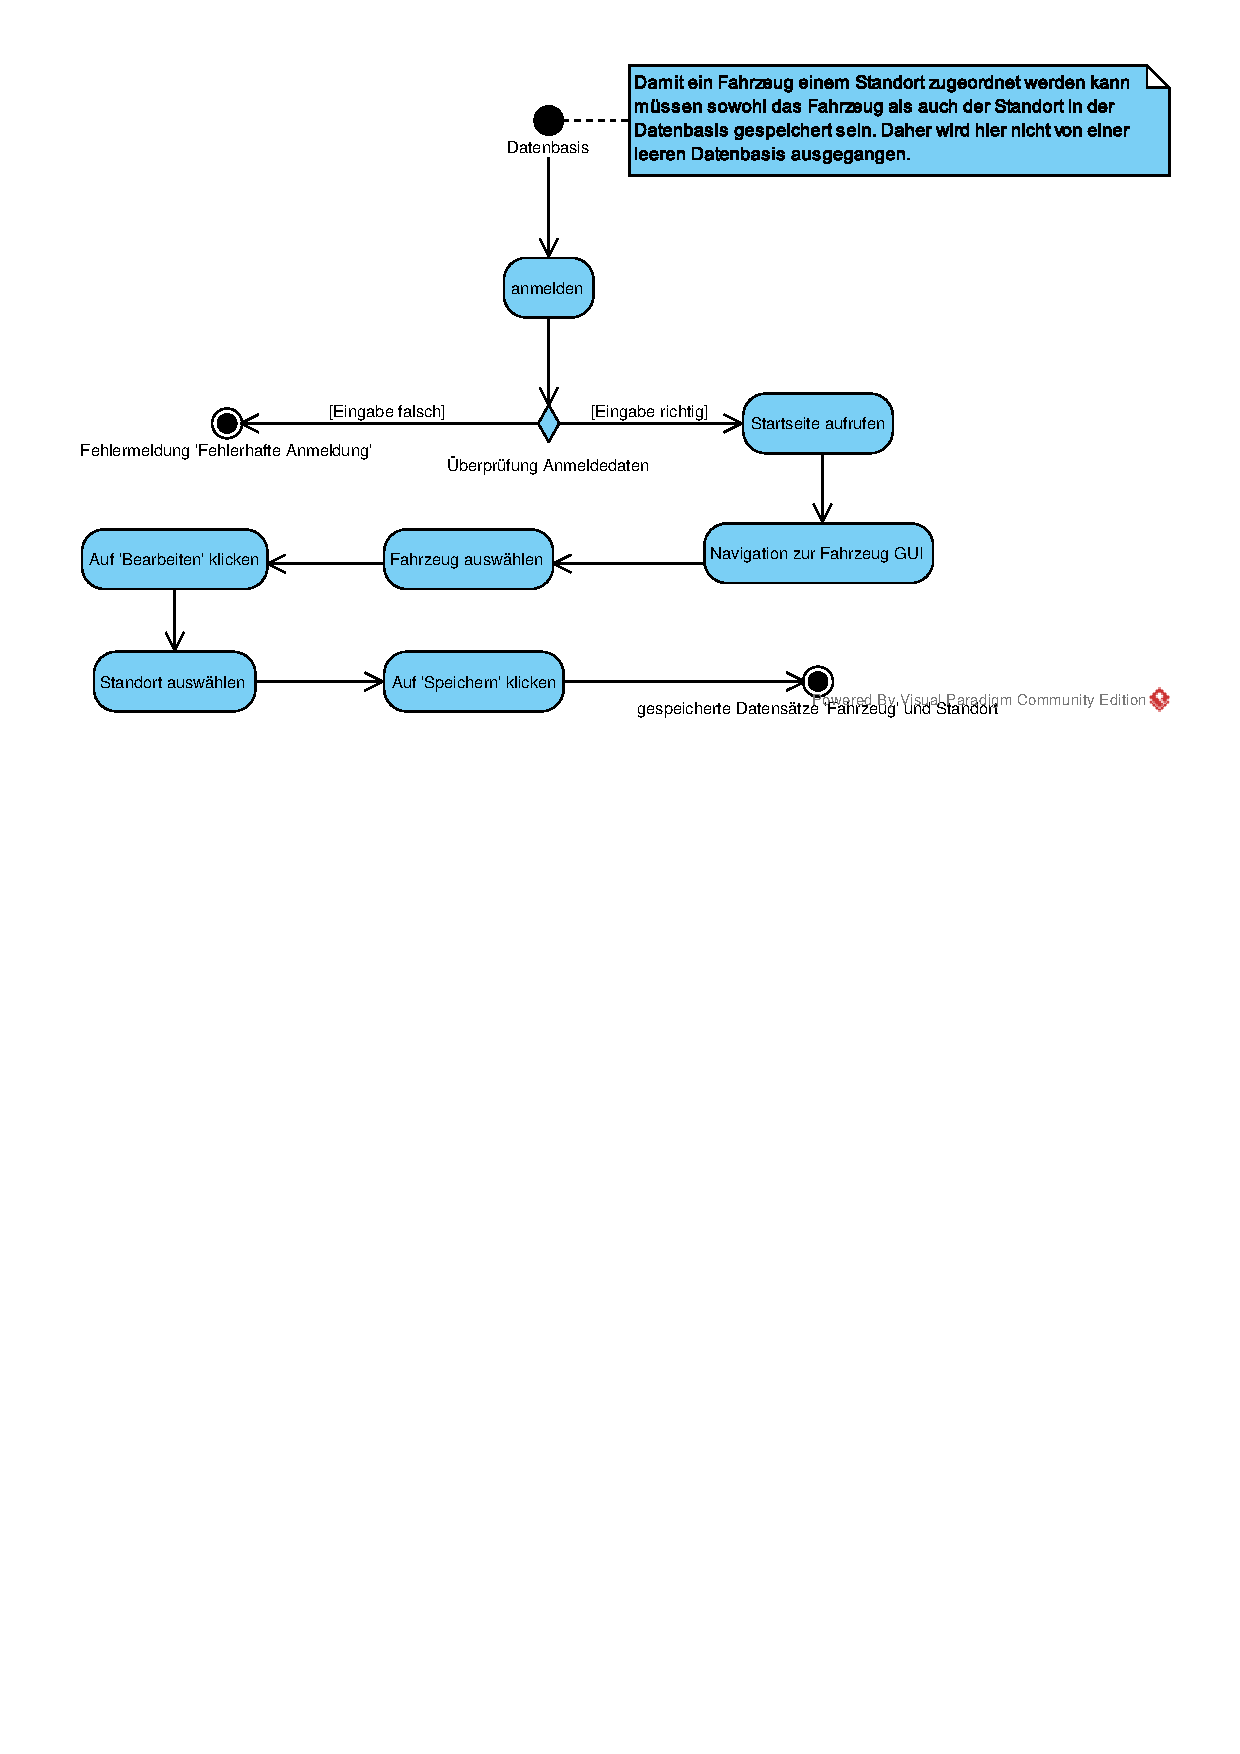
\includegraphics[width=\textwidth, trim = 0cm 11cm 0cm 0cm]{Bilder/Diagramme/FahrzeugStandortZuordnen.pdf}
    \caption{Aktivitätsdiagramm: Fahrzeug einem Standort zuordnen}
    \label{img:fahrzeugzuordnen}
\end{figure}

Nachdem die Standorte und Fahrzeuge angelegt wurden, können die Fahrzeuge einem Standort zugewiesen werden. Die Zuweisung wird in Abbildung \ref{img:fahrzeugzuordnen} dargestellt. Dazu wird davon ausgegangen, dass der Mitarbeiter noch nicht im System angemeldet ist. Daher ist der erste Schritt die Anmeldung im System. Sollte die Eingabe bei der Anmeldung fehlerhaft sein so wird eine Fehlermeldung angezeigt und der Nutzer kann nicht auf die Anwendung zugreifen. Falls die Anmeldung erfolgreich ist, wird dem Nutzer die Startansicht angezeigt. Um nun ein Fahrzeug einem Standort zuzuweisen muss der Nutzer zunächst auf die Fahrzeug-GUI navigieren. Hier kann das Fahrzeug, welches einem Standort zugewiesen werden soll, ausgewählt werden. Nachdem der Nutzer auf 'Bearbeiten geklickt hat, ist die Auswahl eines Standortes möglich. Sobald der Nutzer auf 'Speichern' klickt wird sowohl der Datensatz des Standortes als auch der Datensatz des Fahrzeugs angepasst und gespeichert.


\chapter{Entwurfsklassendiagramm}

Im folgenden Kapitel wird das Entwurfsklassendiagramm (EKD) genauer erklärt. Das EKD erweitert das Analyseklassendiagramm um Pakete, Methoden, Attribute und weitere Elemente, welche für die Umsetzung notwendig sind.

\section{Diagramm}

\begin{figure}[!ht]
    \centering
    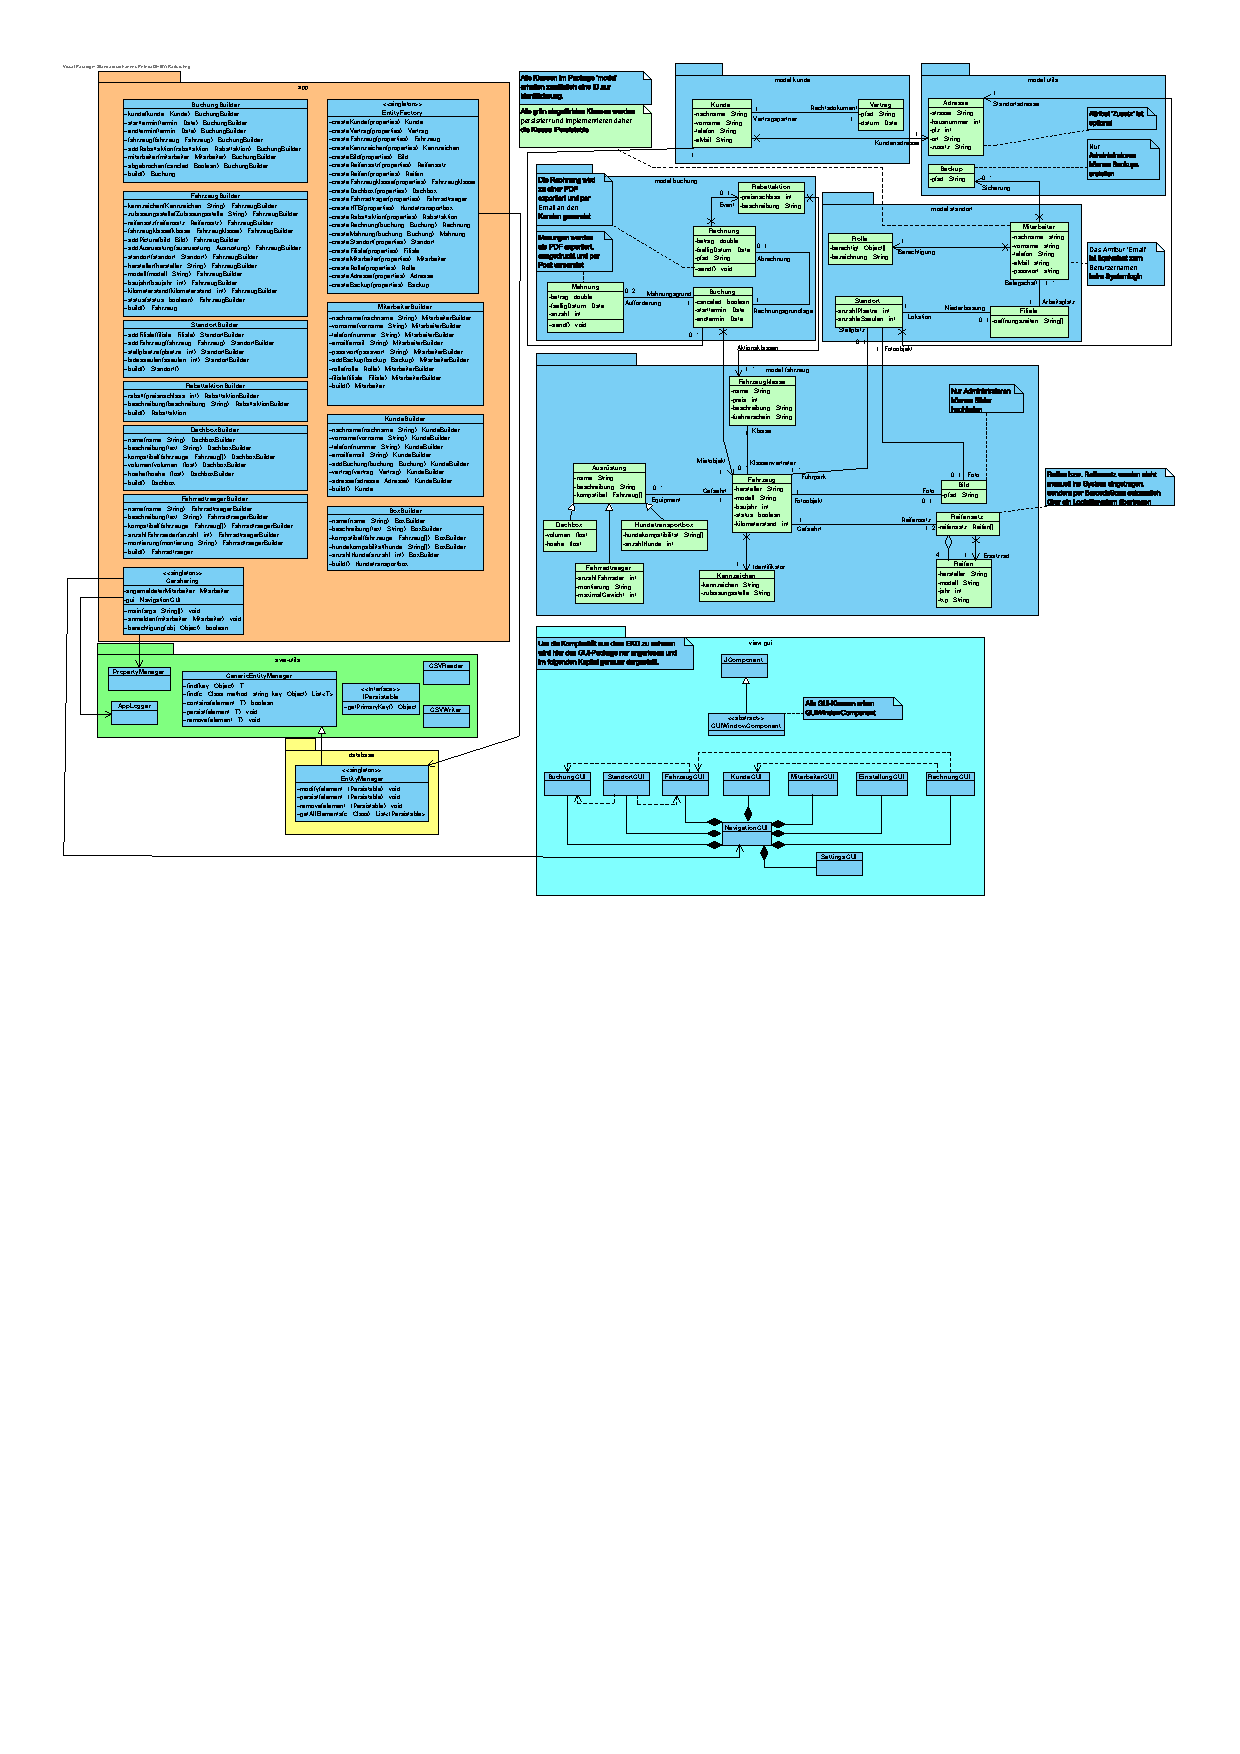
\includegraphics[width=\textwidth, trim = 0cm 14cm 0cm 0cm]{Bilder/Diagramme/Entwurfsklassendiagramm_v2.pdf}
    \caption{Aktivitätsdiagramm: Fahrzeug einem Standort zuordnen}
    \label{img:ekd}
\end{figure}

\newpage

\section{Pakete}

\subsection{model.buchung}

Dieses Paket enthält alle Klassen aus dem Analyseklassendiagramm, welche der Klasse 'Buchung' zugeordent werden können. Dazu gehören die Klassen 'Buchung', 'Rabattaktion', 'Rechnung' und 'Mahnung'. Damit auch die stornierten Buchungen noch eingesehen werden können, verfügt jede Buchung über ein Attribut, welches indiziert, ob die Buchung storniert wurde. Die Rabattaktion verfügt über ein Attribut für den prozentualen Preisnachlass. Die Rechnung ist durch Attribute für den Betrag der Rechnung und deren Fälligkeit definiert. Dazu gibt es eine Methode, um die Rechnung zum Kunden zu senden. Die Mahnung unterscheidet sich bezüglich der Attribute und Methoden nicht von der Rechnung.

\subsection{model.fahrzeug}

Dieses Paket enthält alle Klassen, welche sich auf das Fahrzeug beziehen. Dazu gehören die Klassen 'Fahrzeug', 'Kennzeichen', 'Reifensatz', 'Reifen', 'Fahrzeugklasse' sowie 'Ausrüstung' und die Unterklassen der Ausrüstung ('Dachbox', 'Fahrradträger' und 'Hundetransportbox').
Das Fahrzeug besitzt Attribute, welche Auskunft über den Hersteller, das Baujahr und das Modell geben. Die restlichen Klassen des Paketes verfügen jeweils über Attribute, um das Fahrzeug beziehungsweise den dargestellten Bestandteil des Fahrzeuges genauer zu beschreiben. 

\subsection{model.kunde}

Dieses Paket enthält nur die Klasse 'Kunde' und die Klasse 'Vertrag' da dies bereits alle Klassen sind, welche einen direkten Bezug zum Kunden haben.
Die Klasse 'Vertrag' enthält nur den Pfad, unter welchem der Vertrag gespeichert wurde. Die Klasse 'Kunde' enthält hingegen alle Informationen, welche für die Kontaktierung des Kunden notwendig sind.

\subsection{model.standort}

Dieses Paket enthält alle Klassen, welche einen Standort sowie dessen Mitarbeiter darstellen. Dazu gehören neben der Klasse 'Standort' auch die Klassen 'Filiale', 'Mitarbeiter' und 'Rolle'. Die Rolle definiert dabei auf welche Objekte ein Mitarbeiter zugreifen darf. Der Standort hat als Attribute die Anzahl der Parkplätze und Ladesäulen, welche zur Verfügung stehen und die Filiale besitzt die Öffnungszeiten als Attribut. Der Mitarbeiter wird ähnlich wie der Kunde hauptsächlich durch Kontaktinformationen dargestellt. Jedoch wird außerdem noch das Passwort des Mitarbeiters gespeichert, damit dieser sich bei der Anwendung anmelden kann.

\subsection{model.utils}

In diesem Paket befinden sich Klassen, welche von verschiedenen anderen Klassen verwendet werden. Dazu gehört neben der Klasse 'Adresse' auch die Klassen 'Backup' und 'Bild'.

\subsection{app}

Hier befindet sich zum einen die zentrale Klasse 'Carsharing', welche die Main-Methode für das Starten der Anwendung beinhaltet. Diese Klasse wird als Singleton implementiert. Zum anderen befindet sich hier die 'EntityFactory', welche für das Erzeugen von Instanzen der Klassen aus den Model-Paketen, welche in der Datenbasis gespeichert werden, verantwortlich ist. Für die Buchungen, Fahrzeuge, Standorte, Mitarbeiter, Kunden, Rabattaktionen, Dachboxen, Fahrradträger und Hundetransportboxen werden extra Builder implementiert, da es sich hierbei um besonders komplexe Klassen handelt. 

\subsection{swe-utils}

Dieses Paket enthält eigentlich noch wesentlich mehr Klassen, welche jedoch nicht mit dargestellt werden, da sie für die Anwendung irrelevant sind. Die enthalten Klassen beinhalten den 'CSVReader' und 'CSVWriter', welche im EntityManager für das Speichern der Daten eingesetzt werden. Für diese Persistierung der Daten ist das Interface 'IPersistable' enthalten. Außerdem befindet sich hier auch der 'PropertyManager' und der 'AppLogger'.

\subsection{database}
Dieses Paket beinhaltet nur eine Klasse. Dabei handelt es sich um den generischen 'EntityManager', welcher von der Klasse 'GenericEntityManager' aus dem Paket 'swe-utils' erbt. Diese Klasse wird als Singleton implementiert und ist für die Verwaltung der Entitäten verantwortlich.

\subsection{gui}
Dieses Paket beinhaltet alle Klassen, welche die Benutzeroberfläche betreffen. Dazu gehören neben einer Vielzahl von Klassen, welche auf 'GUI' enden auch die abstrakte Klasse 'GUIComponent' und die Klasse 'JComponent'. 'GUIComponent' erbt hierbei von 'JComponent' und alle auf 'GUI' endenden Klassen erben von 'GUIComponent'. Diese Klassen, welche auf 'GUI' enden, stellen die einzelnen Ansichten der Anwendung dar. Im Sinne der Übersichtlichkeit wurde in diesem Diagramm auf die Detailtiefe bezüglich der Benutzeroberfläche verzichtet. Diese wird im nächsten Kapitel ab Seite \pageref{chapter:gui} genauer beschrieben.

\section{Entwurfsmuster}
Für die Implementierung der Carsharingsoftware verwenden wir verschiedene Entwurfsmuster, welche das Auftreten von Problemen verhindern sollen. Solche Entwurfsmuster sind wiederverwendbare Schablonen zur Problemlösung. Im folgenden Abschnitt werden die verwendeten Entwurfsmuster genauer erläutert und erklärt, wie diese für die Implementierung eingesetzt werden. 

\subsection{EntityManager}
Bezüglich des EntityManagers wurde sich dafür entschieden eine generische Klasse zu implementieren, welche alle gespeicherten Entitäten verwaltet. Dies hat den Vorteil, dass die Verwaltung der Entitäten sehr simpel dargestellt und Implementiert werden kann.

\subsection{Builder}
Für das Erstellen von komplexeren Klassen setzen wir in unserem Entwurf sogenannte Builder ein. Zu diesen Klassen gehören die Buchung, das Fahrzeug, der Standort sowie der Mitarbeiter. Durch den Builder wird ein schrittweises Erstellen von Instanzen dieser Objekte ermöglicht, wodurch die Erstellung dieser Objekte deutlich vereinfacht wird.

\subsection{EntityFactory}
Die EntityFactory wird verwendet, um Instanzen einzelner Klassen zu erstellen. Dazu verfügt die EntityFactory für jede Klasse, für welche eine Instanz erzeugt werden soll, über eine Methode, welche nach der Persistierung des Objektes mithilfe des EntityManagers eine Instanz zurückgibt. Um solche Insatnzen zu erstellen, müssen den Methoden verschiedene Parameter übergeben werden. Diese Parameter werden im Diagramm zur Vereinfachung als 'properties' dargestellt.

\subsection{Singleton}
Ein Singleton stellt sicher, dass es zu einer Klasse nur genau ein einziges Objekt gibt. Diese Singletons werden in unserem Entwurf an verschiedenen Stellen eingesetzt. Bei diesen Stellen handelt es sich um die Klasse 'Carsharing', den EntityManager und die EntityFactory. Mit der Verwendung dieses Entwurfsmusters wird die Verhinderung des Auftretens von Dateninkonsistenzen beabsichtigt.

\subsection{Beobachter}
Mit Beobachtern kann auf die Veränderung von Objekten reagiert werden. Solche Beobachter wurden in unserem Entwurf lediglich passiv implementiert. Das heißt, dass die Beobachter nicht aktiv den Zustand eines konkreten Objektes abfragen, sondern nur dann benachrichtigt werden , wenn Änderungen aufgetreten sind. Dadurch ergibt sich eine größere Vielfalt der Abstraktionsmöglichkeiten und die Wiederverwendbarkeit von einzelnen Komponenten.

\subsection{Kompositum}
Das Kompositum wird genutzt um Teil-Ganzes-Hierachien darzustellen. In unserem Entwurfsklassendiagramm wird dies zum einem bei der Modellierung des Reifensatzes eines Fahrzeuges und zum anderen auch bei der Modellierung der Benutzeroberfläche genutzt. Ein Reifensatz besteht hierbei aus vier oder fünf Reifen, je nachdem, ob ein Ersatzrad vorhanden ist und bei der Benutzeroberfläche sind die Unteransichten ein Teil der Hauptansicht.
\chapter{GUI-Entwurf}
\label{chapter:gui}

Eine Software kann noch so gut geplant und durchstrukturiert sein, wenn die Benutzeroberfläche jedoch unübersichtlich ist und nicht bedient werden kann, dann ist der gesamte Rest hinfällig. Daher ist es nötig sich bereits im Vorfeld eine mögliche Front-End-Gestaltung zu überlegen. In Anbetracht der Tatsache, dass der Programmentwurf in Java umgesetzt werden wird, haben wir beim GUI-Entwurf auf die Gestaltung von zu umständlichen und modernen Bestandteilen, wie man sie heute auf den meisten Webseiten sehen kann, verzichtet und uns auf die grundlegenden Bestandteile fokussiert. 


Übergeordnet soll in der gesamten Anwendung ein einheitliches Design vorliegen. Darum haben wir uns bereits zu Beginn auf ein Farbschema abgestimmt. Aus unerklärlichen Gründen hat uns ein rötlich-rosa Farbschema überzeugt, sodass die Farben (in Hexwerten) \textbf{\#DE639A}, \textbf{\#E388B1}, \textbf{\#D7A6B3}, \textbf{\#F1E2E2}, \textbf{\#707070} ihre Anwendung fanden. 

\section{Fahrzeuge verwalten}

Grundsätzlich sollen alle Verwaltungsbereiche der Anwendung den selben oder einen sehr ähnlichen Aufbau haben, damit auch Mitarbeiter ohne besondere IT-Kenntnisse die Anwendung verwenden können. Neben einer Headline, die eine Überschrift und das Firmenlogo präsentiert, gibt es an dem linken Bildschirmrand die Navigationsleiste, mit der Mitarbeiter sich durch die unterschiedlichen Verwaltungsaufgaben klicken können. Der Hauptbereich einer jeden Seite wird in zwei Felder aufgeteilt. Das linke Feld besteht aus einer Liste, in der alle Einträge zum betroffenen Verwaltungsobjekt angezeigt werden, in diesem Fall alle Fahrzeuge. Bei Auswahl eines Fahrzeuges erscheint im rechten Feld eine Detail-Anzeige aller nötiger Informationen, die es zu dem Listeneintrag gibt. Neben einem Filter- und Suchfeld ist natürlich auch die Manipulation der Datensätze vorgesehen, sodass man einerseits neue Fahrzeuge anlegen kann. Wie in vorhergehenden Analysen angedacht gibt es dabei einerseits einen einfachen Button mit 'anlegen' und für erfahrenere Nutzer einen Button mit '+'. Sollte ein Listeneintrag ausgewählt sein, ist auch die Bearbeitung oder das Löschen des ausgewählten Datensatzes mittels entsprechender Buttons möglich. 

\newpage

\begin{figure}[!ht]
    \centering
    \includegraphics[width=\textwidth]{Bilder/Mockup/Web 1920 – 3.png}
    \caption{Mock-Up: Liste an Fahrzeugen}
    \label{mu:fahrzeugliste}
\end{figure}

\begin{figure}[!ht]
    \centering
    \includegraphics[width=\textwidth]{Bilder/Mockup/Web 1920 – 4.png}
    \caption{Mock-Up: Detailansicht eines Fahrzeugs}
    \label{mu:fahrzeugdetails}
\end{figure}

\newpage

\subsection{Fahrzeug löschen}

Die Interaktion zum Löschen des ausgewählten Fahrzeug-Datensatzes erfolgt über ein einfaches Pop-Up-Fenster. Der Anwender muss dieses Bestätigen, wenn er den Datensatz löschen möchte, um versehentliches Löschen auszuschließen. Nach dem Löschen wird der Anwender auf die Fahrzeug-Startseite zurückverwiesen, jedoch wird in der Liste der gelöschte Eintrag entfernt. 


\begin{figure}[!ht]
    \centering
    \includegraphics[width=\textwidth]{Bilder/Mockup/Web 1920 – 5.png}
    \caption{Mock-Up: Löschen eines Fahrzeugs}
    \label{mu:loeschen}
\end{figure}

\newpage

\subsection{Fahrzeug bearbeiten}

Das Bearbeiten eines Datensatzes ist so einfach wie möglich gestaltet. Der einzige Unterschied von der Bearbeitungs-GUI zur Detail-GUI ist, dass alle Felder, die bearbeitet werden können sollen, entweder zu einem Eingabefeld oder einer Drop-Down-Liste werden. Im folgenden Beispiel werden nur die Felder 'Reifen' und 'Ausrüstung' bearbeitbar. Da es sehr unwahrscheinlich ist, dass sich bei einem bereits vorhandenen Fahrzeug der Hersteller, das Modell, die Fahrzeugklasse oder das Baujahr ändern, soll es nicht bearbeitbar sein. Informationen wie Preis, Kilometerstand werden vom System vorgegeben und einfach nur angezeigt. Es ist aber möglich bei einem Fahrzeug die Reifen zu wechseln, z.B. von Sommer- auf Winterreifen oder auch die Ausrüstung zu ändern, da z.B. eine Dachbox angebracht und wieder abmontiert werden kann. Da bei beiden Feldern keine freie Eingabe möglich sein soll, sondern nur aus Vorhandenem ausgewählt werden soll, ist die Bearbeitung mittels Checkbox-Liste vorgesehen. 


\begin{figure}[!ht]
    \centering
    \includegraphics[width=\textwidth]{Bilder/Mockup/Web 1920 – 9.png}
    \caption{Mock-Up: Bearbeiten eines Fahrzeugs}
    \label{mu:bearbeiten}
\end{figure}

\newpage

\subsection{Fahrzeug anlegen}

Die letzte ausstehende Interaktionsmöglichkeit ist das Anlegen eines neuen Fahrzeugs. Auch hier wird nur die rechte Fläche für das Erstellen verwendet. Wie beim Bearbeiten erfolgt die Eingabe über einfache Eingabefelder oder Listen. Da das Fahrzeug noch nicht angelegt wurde, hat es auch keinen Status. Informationen über Hersteller, Modell, Baujahr und Kilometerstand sind frei einzutragen, wobei es ggf. auch möglich ist Felder wie Hersteller und Baujahr als Auswahlliste zu realisieren. Die Einordnung in die Klasse erfolgt ausschließlich über eine Auswahlliste und mit Auswahl eines Eintrages wird auch der Preis des Fahrzeuges gesetzt. Reifen und Ausrüstung sind Checkbox-Listen. 

Als Vorbereitung auf die Webanwendung für Kunden und zur optisch schöneren Darstellung in der Anwendung ist es möglich ein Bild vom Fahrzeug hochzuladen. Diese Aktion ist nur für einen Admin möglich und kann jederzeit nachgeholt werden. Sollte kein Bild beim Anlegen hochgeladen werden, wird ein neutrales Platzhalter-Foto verwendet. 

\begin{figure}[!ht]
    \centering
    \includegraphics[width=\textwidth]{Bilder/Mockup/Web 1920 – 10.png}
    \caption{Mock-Up: Anlegen eines Fahrzeugs}
    \label{mu:anlegen}
\end{figure}

\section{Standorte verwalten}

Es ist erwünscht, dass von mindestens zwei wesentlichen GUI-Komponenten Skizzen erstellt werden. Neben der 'Verwaltung von Fahrzeugen' wird die 'Verwaltung von Standorten' genauer ausgebaut. Der Seitenaufbau ist identisch zur Fahrzeugverwaltung. Auf der Standort-Startseite befindet sich auf der linken Hälfte eine Liste mit allen eingetragenen Firmen-Standorten. Auch die zusätzlichen Interaktionsmöglichkeiten wie Suchen, Filtern und Anlegen sind identisch zu anderen Verwaltungsbereichen. Die rechte Seite der Hauptfläche wird von einer interaktiven Karte eingenommen (möglich wäre z.B. eine Einbindung von google.de/maps), auf der alle Standorte mit Markierungen eingetragen sind. 

\begin{figure}[!ht]
    \centering
    \includegraphics[width=\textwidth]{Bilder/Mockup/Web 1920 – 11.png}
    \caption{Mock-Up: Liste an Standorten}
    \label{mu:standortliste}
\end{figure}


Sofern man eine Markierung auf der Karte oder einen Listeneintrag auswählt, wird man zu einer Standort-Detail-Seite geleitet. Ebenfalls identisch vom Aufbau zur Fahrzeug-Detail-Ansicht findet man auf der rechten Seite eine detailierte Darstellung des Standortes. Dazu gehören Standortadresse, Parkplatzanzahl, das Vorhandensein von E-Ladesäulen und einer Filiale und ggf. deren Öffnungszeiten. Ebenfalls ist ein Foto angedacht. Die Fläche auf der linken Bildschirmseite ist eine Liste, doch dieses Mal werden in dieser Liste alle Fahrzeuge angezeigt, die normalerweise am Standort vorhanden sind.  

\begin{figure}[!ht]
    \centering
    \includegraphics[width=\textwidth]{Bilder/Mockup/Web 1920 – 12.png}
    \caption{Mock-Up: Detailansicht von Standorten}
    \label{mu:standortdetails}
\end{figure}








Der Nutzer soll die Möglichkeit haben das Design der Benutzeroberfläche auf ein 'Dark Theme' umzustellen. Durch die Auswahl des 'Dark Themes' soll die Benutzeroberfläche der Anwendung dunkler dargestellt werden. Dazu haben wir uns für folgendes Farbschema entschieden (siehe Abbildung \ref{mu:darkmode}).

\begin{figure}[!ht]
    \centering
    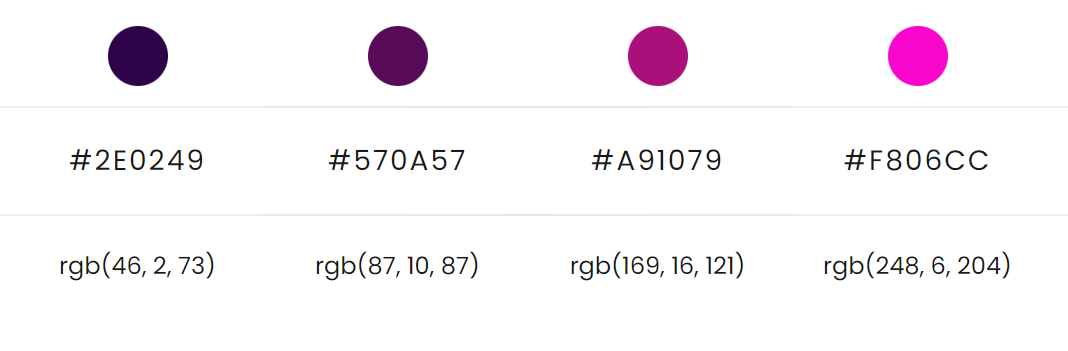
\includegraphics[width=\textwidth]{Bilder/Mockup/colorscheme_darkmode.PNG}
    \caption{Dark Theme Farbschema}
    \label{mu:darkmode}
\end{figure}
\chapter{Besonderheiten}
Im folgenden Kapitel werden dem Leser die Besonderheiten der entwurfenen Software näher gebracht.

\section{Detailtiefe}
Damit der Kunde bei der Buchung eines Fahrzeuges so viele Informationen wie nur möglich über das Mietobjekt erhält, wurde vor allem bei der Modellierung des Fahrzeuges auf eine große Detailtiefe geachtet. Dies ermöglicht nicht nur dem Kunden eine bessere Entscheidung über das passende Fahrzeug zu treffen, sondern vereinfacht auch die Instandhaltung und die Bestandsaufnahme für das Carsharing selbst, da alle wichtigen Informationen zu den Fahrzeugen abgebildet werden können. Dazu zählen unteranderem die Reifen, welche zum einen als Reifensatz aber auch als einzelne Reifen modelliert wurden. Außerdem wurde jegliche Ausrüßtung der Fahrzeuge durch dedizierte Klassen detailliert beschrieben. Auch die Wartungen können problemlos dargestellt werden, indem eine Buchung für die Werkstatt angelegt wird.

Damit die Anwendung im Einsatz vollfunktional ist, wurden auch Rabattaktionen mit eingebunden, welche es dem Carsharing erlauben die Preise für einzelne Fahrzeugklassen temporär zu senken. Dies wird automatisch mit in die Rechnung für den Kunden einbezogen. Diese Rechnungen werden auch automatisch durch unser System versendet und falls diese nicht bezahlt werden sollten, stehen wir bereits in engem Kontakt mit der schweizerischen Nationalbank (SNB) um ein Reibungsloses einfrieren des Bankkontos zu ermöglichen.


\section{Benutzeroberfläche}
Auf die Detailreiche der modellierten Benutzeroberfläche ist besondere Aufmerksamkeit zu werfen, da sich hier an sogar an einer Mitarbeiterumfrage bezüglich der Farbauswahl orientiert wurde. Für die Benutzeroberfläche wurden insgesamt neun unterschiedliche Ansichten entwurfen, welche als Orientierung für die Implementierung dienen. Hierbei wurde jeder Schlüsselaspekt der Anwendung und noch mehr ersichtlich, indem neben dem Anlegen von Buchungen sowie die Übersichten der Fahrzeuge und Buchungen auch die Detailansichten für sowohl Fahrzeuge als auch Standorte bereits modelliert wurden. Zudem ist für die Fahrzeuge jeweils eine Ansicht zum Anlegen, Löschen und Bearbeiten erstellt wurden. Dabei wurden auch Details wie das Logo, oder eine Karte für die Standorte berücksichtigt. Ebenfalls berücksichtigt wurde das hohe Durchschnittsalter beziehungsweise der hohe Anteil der digitalen Analphabeten unter den Mitarbeitern des Kunden. Um diesen prozentual gesehen nicht unerheblichen Teil der Mitarbeiter einen einfachen Umgang mit der Anwendung zu gewährleisten, wurde besonders auf Benutzerfreundlichkeit geachtet. Dazu wurden extra Icons zusätzlich zum Text in der Navigation hinzugefügt. Bei der Navigation wurde zudem komplett auf die Verwendung von Transaktionen verzichtet, sodass alles über die Navigationsleiste am linken Fensterrand erreichbar ist. Außerdem wurde darauf geachtet, dass alle Funktionen mit nicht mehr als drei Klicks zu erreichen sind. Die wohl wichtigste Designentscheidung im Bezug auf das hohe Durchschnittsalter ist aber wohl die dreifache Abfrage, ob sich der Nutzer sicher ist, ob er das Element löschen möchte. Denn im höheren Alter kann es durchaus schon mal vorkommen, dass man mal mit der Maus ausrutscht und ausversehen etwas löscht oder kontroverse Statements postet (siehe Beatrix von Storch). Um dies zu verhindern fragen wir lieber drei mal nach, bevor etwas wirklich gelöscht wird. Des Weiteren wird in den Formularen überall wo es möglich ist ein Auswahlfeld anstelle einer Texteingabe verwendet, damit die Mitarbeiter nicht die kleinen Tastaturtasten suchen müssen. Dadurch werden zahlreiche Tippfehler präventiv vermieden. Eine weitere Designentscheidung für den Komfort bei der Bedienung ist, dass alles in einem Fenster dargestellt wird und keine weiteren sinnlosen Fenster geöffnet werden. So werden nur für  Löschbestätigungen Popups verwendet.

Die erwähnten Ansichten wurden alle als Teil eines Interaktiven Prototyps entwickelt. Der Prototyp wurde mithilfe von Adobe XD erstellt und ist mit angehängt. Um den Prototyp öffnen zu können ist Adobe XD vorausgesetzt.

Da die Mitarbeiter des Carsharings verschiedene Vorlieben bezüglich der Optik haben, wurden verschiedene Einstellungsmöglichkeiten für die Benutzeroberfläche eingeplant. So sind die Schriftart, Textgröße und Fenstergröße anpassbar auf die Ansprüche des entsprechenden Mitarbeiters. Zusätzlich steht die Möglichkeit zur Verfügung, zwischen 'Light Theme' und 'Dark Theme' zu wechseln. Dadurch soll es möglich sein, dass jeder Mitarbeiter die Anwendung individuell nach seinen Bedürfnissen einrichten kann.

\section{Pseudocode}
Sowohl für das Anlegen einer Buchung, als auch das Anlegen eines Standortes mit Fahrzeugen wurde, neben der Dokumentation durch Sequenzdiagramme beziehungsweise Aktivitätsdiagramme, bereits detaillierter Pseudocode geschrieben. Dieser bildet den Programmablauf genaustens ab und erleichtert somit die Implementierung erheblich. Dabei wurde auch auf Modularisierung geachtet, indem einzelne Programmabschnitte gezielt in eigene Methoden ausgelagert wurden. Dadurch wird der Ablauf noch einfacher verständlich und auf einzelne Teilschritte heruntergebrochen.

\section{Übersichtlichkeit}
Um die Komplexität der Modellierung zu reduzieren, wurde sich dazu entschieden bestimmte Funktionen zu vereinfachen beziehungsweise zusammenzufassen. So wird zum Beispiel jeglicher Import und Export von Daten mithilfe der Klasse 'Backup' dargestellt. Ein weiteres Beispiel ist die Klasse 'Buchung', welche sowohl für die Termine der Kunden als auch für die Wartungstermine bei der Werkstatt verwendet wird. Dadurch wird auf unnötige Komplexität beim Entwurf der Software verzichtet und eine einfachere Bedienung durch weniger Menüs gewährleistet.

\section{Kundenorientierung}
Bei der Planung der Software wurde sich nicht nur an den bedürfnissen der Mitarbeiter des Carsharings orientiert, sondern auch an den Bedürfnissen der Kunden. Dies merkt man zum einen an der bereits erwähnten Detailtiefe, welche dem Kunden so viele Informationen wie möglich zu jedem Fahrzeug bereitstellt und zum anderen an der Reservierungsfunktion. Wenn ein Kunde ein Fahrzeug buchen möchte, wird ein Zeitstempel im System hinterlegt, welcher das Fahrzeug für 15 Minuten reserviert, sodass kein anderer Kunde das Fahrzeug in diesem Zeitraum buchen kann. Dadurch wird zusätlich noch verhindert, dass zwei Mitarbeiter das gleiche Fahrzeug gleichzeitig buchen.  


% ---- Literaturverzeichnis
\cleardoublepage

% ---- Anhang
\appendix
%\clearpage
%\pagenumbering{Roman}  % römische Seitenzahlen für Anhang

\newpage
\end{document}
